%!TEX root = ../thesis.tex
%*******************************************************************************
%*********************************** Fourth Chapter *****************************
%*******************************************************************************


\chapter{Results and analysis}  %Title of the Fourth Chapter

\ifpdf
     \graphicspath{{Figs/Chapter4/}}
\else
    \graphicspath{{Chapter4/Figs/Vector/}{Chapter4/Figs/}}
\fi

This chapter discusses three hypotheses examined in the thesis, including the application of training algorithm optimisations to recursive neural tensor networks (NTNs), compensating for covariate shift introduced by hypernetworks during convolutional tensor factorisation, and finally the intialisation of entity and relation embeddings using pre-trained word vectors. 


%********************************** %Recursive Neural Tensor Networks  **************************************

\section{Recursive neural tensor networks}

\subsection{Baseline training algorithm}
\textbf{Model summary.} This model is inspired by recursive networks (RCNs). The NTN is a bilinear tensor product between the subject, predicate and object, added to a RCN composition of the subject and object. It computes a relational score between two entities. 

\noindent \textbf{Contrastive max-margin loss.} The contrastive max-margin loss is used to train the NTN model. A relational score is computed for the target triple containing a subject, predicate and object. A relational score is then computed for the same subject and predicate, along with a non-related entity randomly selected and presented as a corrupt object. Relational scores in the range $ (-1, \; 1) $ are produced for the target and corrupt objects respectively. The training task is to compute a large value for the target score, and small value for the corrupt score. The computed loss is backpropagated through the network to update model parameters. \par

\noindent \textbf{Experimental setup.} We use the WordNet \unskip ~\citep{miller1995wordnet} and Freebase \unskip ~\citep{bollacker2008freebase} link prediction benchmark datasets.\ WordNet is a lexical database for English, and a taxonomy with hypernym (is - a) relationships, and synonym sets. Freebase is a large collaborative knowledge base consisting of data about the world composed mainly by its community members. It was an online collection of structured data harvested from many sources, including user-submitted wiki contributions. Visualisations of the respective knowledge graphs (KGs), as well as a sample of resource description framework (RDF) triple encoded facts, is presented in Figures 4.1 to 4.4. Property counts for the respective KGs are presented in Tables 4.1 and 4.2. \par

\begin{figure}[H]
   	\centering
    	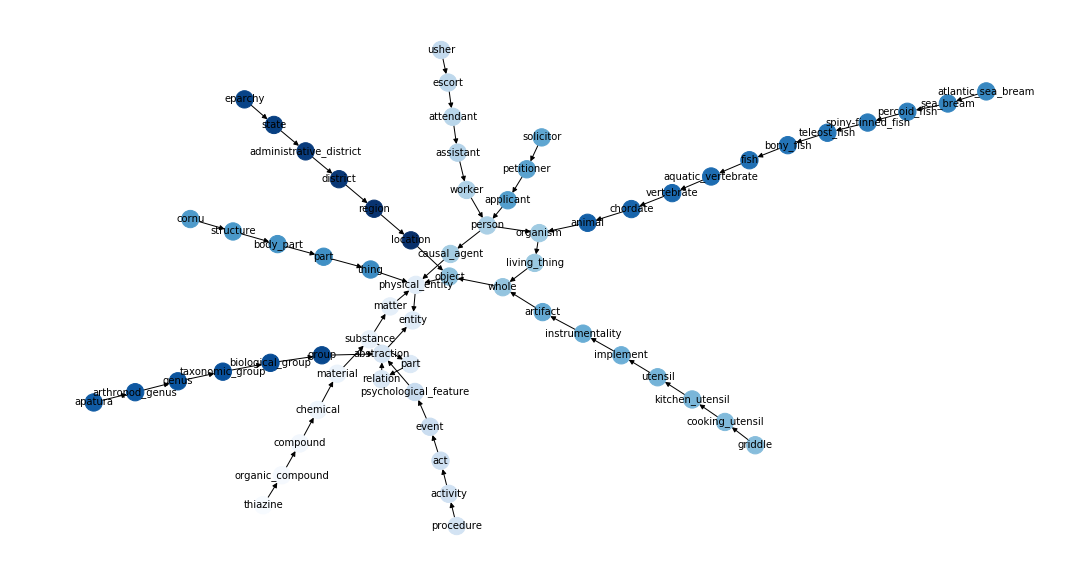
\includegraphics[width=0.9\textwidth, height=0.5\textwidth]{Wordnet}
	\captionsetup{justification=centering}
	\caption{A subset of WordNet facts structured as a KG. Entities are nodes, and relations are edges, where a fact is encoded as an RDF triple.}
\end{figure}

\begin{figure}[H]
   	\centering
    	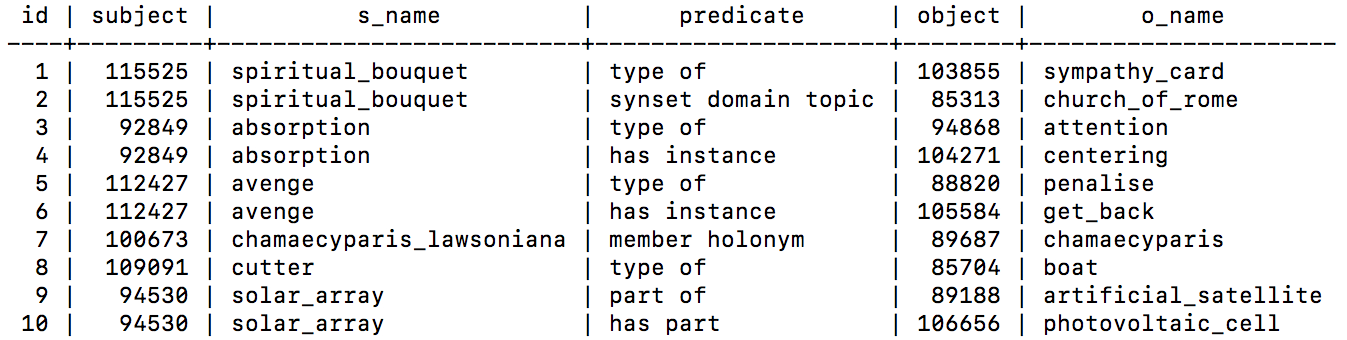
\includegraphics[width=0.9\textwidth, height=0.3\textwidth]{wordnet_fact_sample}
	\captionsetup{justification=centering}
	\caption{A sample of RDF triples from the WordNet KG.}
\end{figure}

\begin{figure}[H]
   	\centering
    	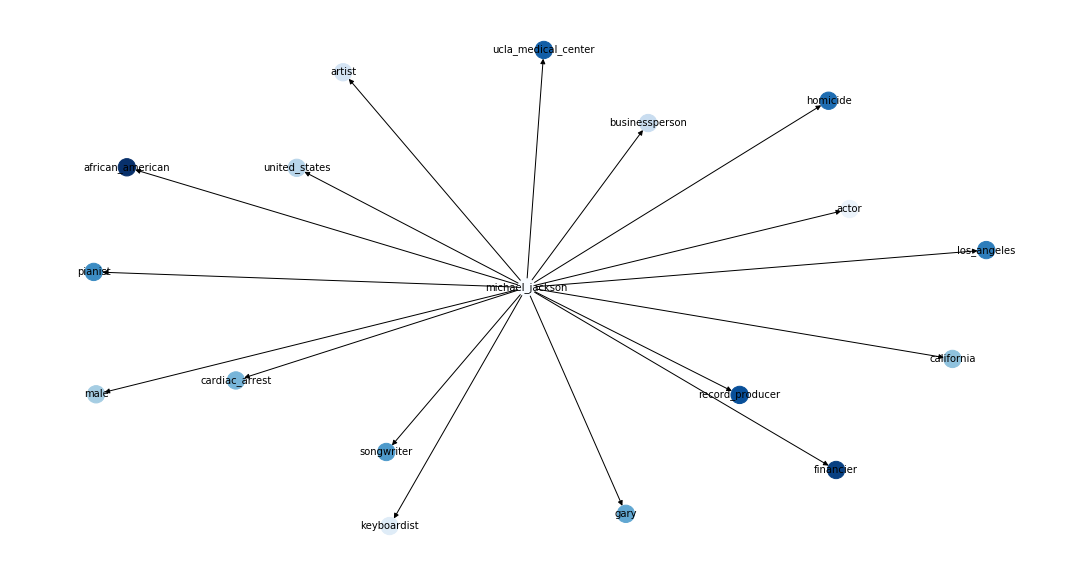
\includegraphics[width=0.9\textwidth, height=0.5\textwidth]{Freebase}
	\captionsetup{justification=centering}
	\caption{A subset of Freebase facts structured as a KG. Due to the size of Freebase, a subset of facts is presented, where "Michael Jackson" is the subject.}
\end{figure}

\noindent 

\begin{figure}[H]
   	\centering
    	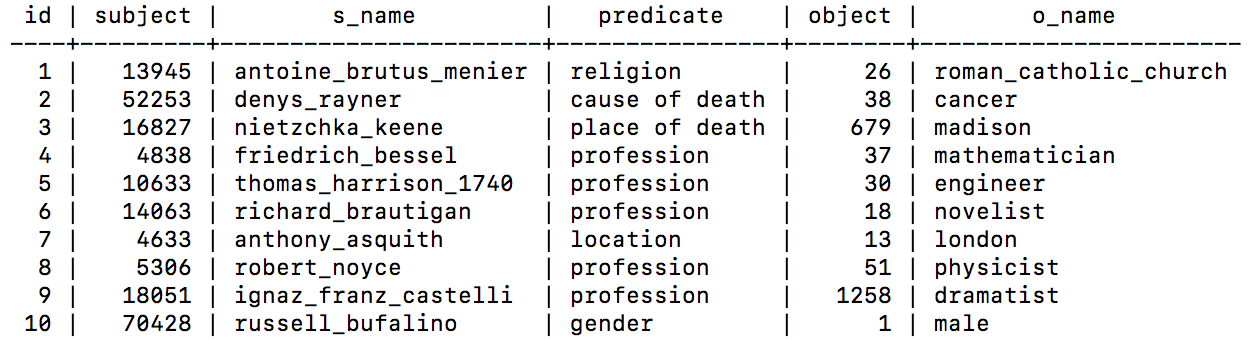
\includegraphics[width=0.9\textwidth, height=0.3\textwidth]{freebase_fact_sample}
	\captionsetup{justification=centering}
	\caption{A sample of RDF triples from the Freebase KG.}
\end{figure}

\noindent We use the TensorFlow framework  \unskip~\citep{abadi2016tensorflow} to implement our improved NTN training algorithm. This algorithm builds upon of the NTN model introduced by Chen, et al. \unskip ~\citep{socher2013reasoning} and reimplemented in TensorFlow by Doss et al. \unskip ~\citep{Doss2015}. Pre-trained word vectors are used to initialise entity and relational embeddings for model training. The embedding parameters are adjusted during training to generate latent representations specific to the KG. \par

\begin{table}[H]
	\parbox{.5\linewidth}{
		\centering
		\begin{tabular}{lllllllllll}
  			\textbf{Property} & \textbf{Count}  \\
  			\hline
  			subjects & 38,696  \\
  			predicates & 11  \\
  			triples & 136,611  \\
			&
		\end{tabular}
		\captionsetup{justification=centering}
		\caption{Counts of WordNet KG elements.}
		}
	\hfill
	\parbox{.5\linewidth}{
		\centering
		\begin{tabular}{lllllllllll}
  			\textbf{Property} & \textbf{Count}  \\
  			\hline
  			subjects & 75,043   \\
  			predicates & 13  \\
  			triples & 375,499  \\
			&
		\end{tabular}
		\captionsetup{justification=centering}
		\caption{Counts of Freebase KG elements.}
		}
\end{table}


%********************************** %Predicate  **************************************

\noindent Summary statistics of the respective KG RDF formalism are presented in Figures 4.5 to 4.7, and Tables 4.3 and 4.8. \par

\bigskip

\begin{figure}[H]
	\begin{subfigure}[b]{.5\linewidth}
   		\centering
    		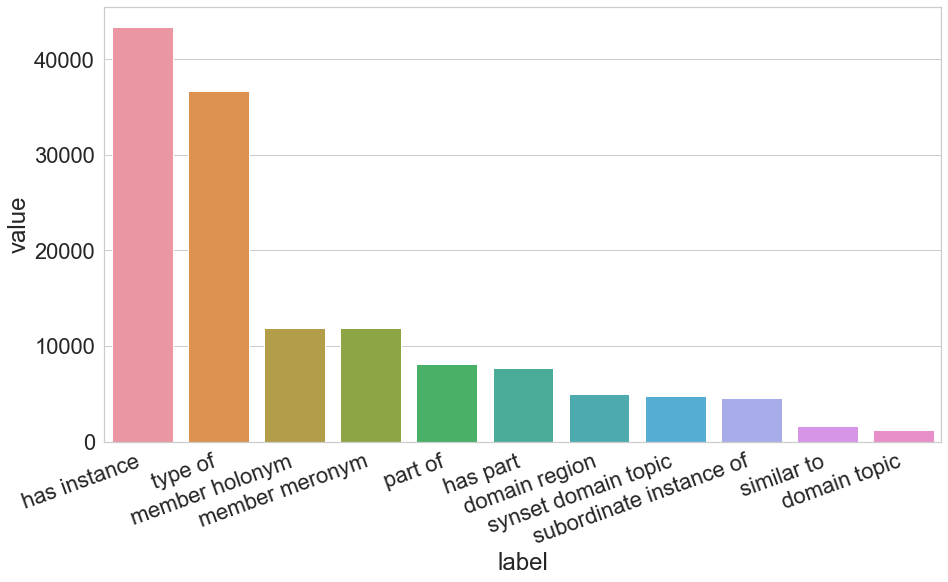
\includegraphics[width=1.0\linewidth, height=0.7\linewidth]{Wordnet_Predicate_Counts}
		\captionsetup{justification=centering}
		\caption{WordNet}
	\end{subfigure}
	\begin{subfigure}[b]{.5\linewidth}
   		\centering
		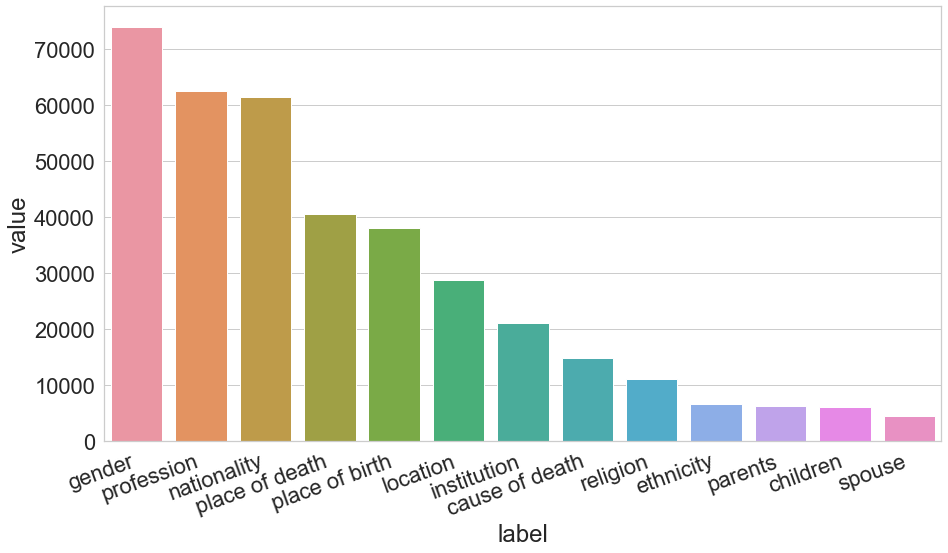
\includegraphics[width=1.0\linewidth, height=0.7\linewidth]{Freebase_Predicate_Counts}
		\captionsetup{justification=centering}
		\caption{Freebase}
	\end{subfigure}
	\captionsetup{justification=centering}
	\caption{KG predicate distribution. The number of times each predicate takes part in a KG fact.}
\end{figure}

\begin{table}[H]
	\parbox{.5\linewidth}{
		\centering
		\begin{tabular}{lllllllllll}
  			\textbf{Statistic} & \textbf{Value}  \\
  			\hline
			Count & 11 \\
			Max & 43,312  \\
			Min & 1,229  \\
  			Median & 7,705  \\
  			IQR & 7,257.5  \\
				&
		\end{tabular}
		\captionsetup{justification=centering}
		\caption{WordNet predicate statistics.}
		}
	\hfill
	\parbox{.5\linewidth}{
		\centering
		\begin{tabular}{lllllllllll}
  			\textbf{Statistic} & \textbf{Value}  \\
  			\hline
			Count & 13 \\
			Max & 73,897  \\
			Min & 4, 464  \\
  			Median & 21,149  \\
  			IQR & 34,033  \\
				&
		\end{tabular} 
		\captionsetup{justification=centering}
		\caption{Freebase predicate statistics.}
		}
\end{table}


%********************************** %Subject **************************************

\begin{figure}[H]
	\begin{subfigure}[b]{.5\linewidth}
   		\centering
    		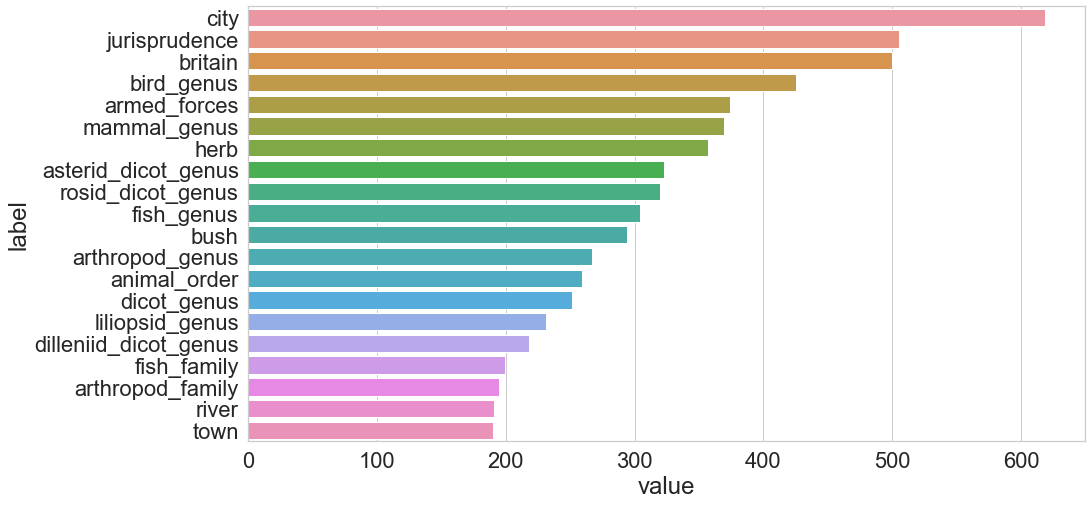
\includegraphics[width=1.0\linewidth, height=0.7\linewidth]{Wordnet_Subject_Counts}
		\captionsetup{justification=centering}
		\caption{WordNet}
	\end{subfigure}
	\begin{subfigure}[b]{.5\linewidth}
   		\centering
		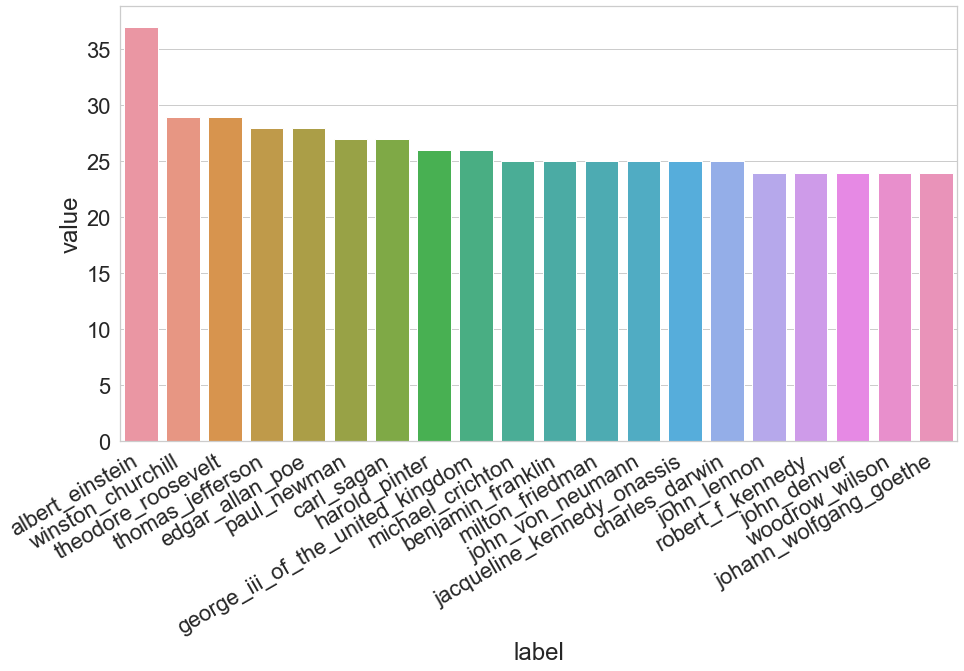
\includegraphics[width=1.0\linewidth, height=0.7\linewidth]{Freebase_Subject_Counts}
		\captionsetup{justification=centering}
		\caption{Freebase}
	\end{subfigure}
	\captionsetup{justification=centering}
	\caption{KG subject distribution. The number of times each subject takes part in a KG fact.}
\end{figure}

\begin{table}[H]
	\parbox{.5\linewidth}{
		\centering
		\begin{tabular}{lllllllllll}
  			\textbf{Statistic} & \textbf{Value}  \\
  			\hline
			Count & 32,720 \\
			Max & 619 \\
			Min & 1 \\
  			Median & 2 \\
  			IQR & 2 \\
				&
		\end{tabular}
		\caption{WordNet subject statistics.}
		}
	\hfill
	\parbox{.5\linewidth}{
		\centering
		\begin{tabular}{lllllllllll}
  			\textbf{Statistic} & \textbf{Value}  \\
  			\hline
			Count & 67,393 \\
			Max & 37 \\
			Min & 1 \\
  			Median & 5 \\
  			IQR & 4 \\
				&
		\end{tabular}
		\caption{Freebase subject statistics.}
		}
\end{table}


%********************************** %Object  **************************************

\begin{figure}[H]
	\begin{subfigure}[b]{.5\linewidth}
   		\centering
    		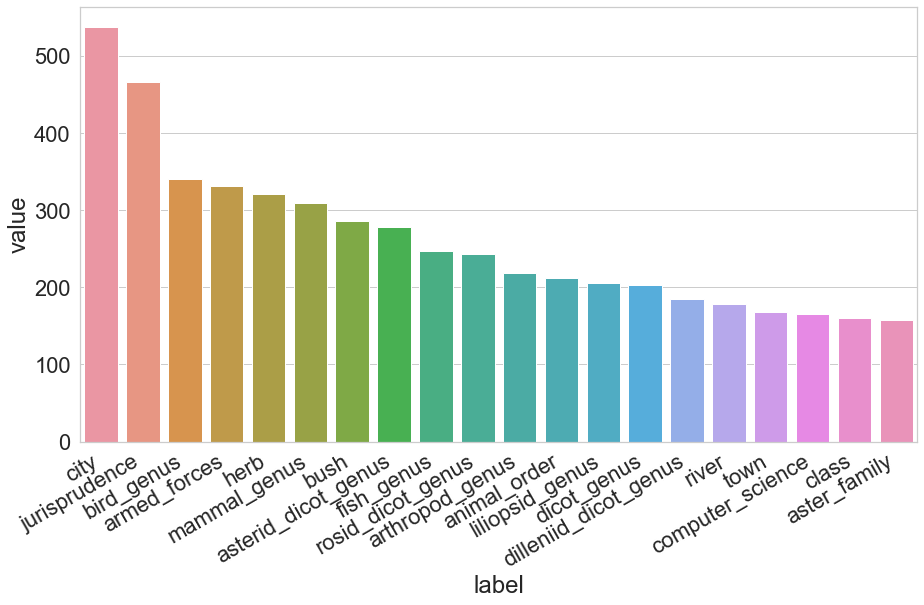
\includegraphics[width=1.0\linewidth, height=0.7\linewidth]{Wordnet_Object_Counts}
		\captionsetup{justification=centering}
		\caption{WordNet}
	\end{subfigure}
	\begin{subfigure}[b]{.5\linewidth}
   		\centering
		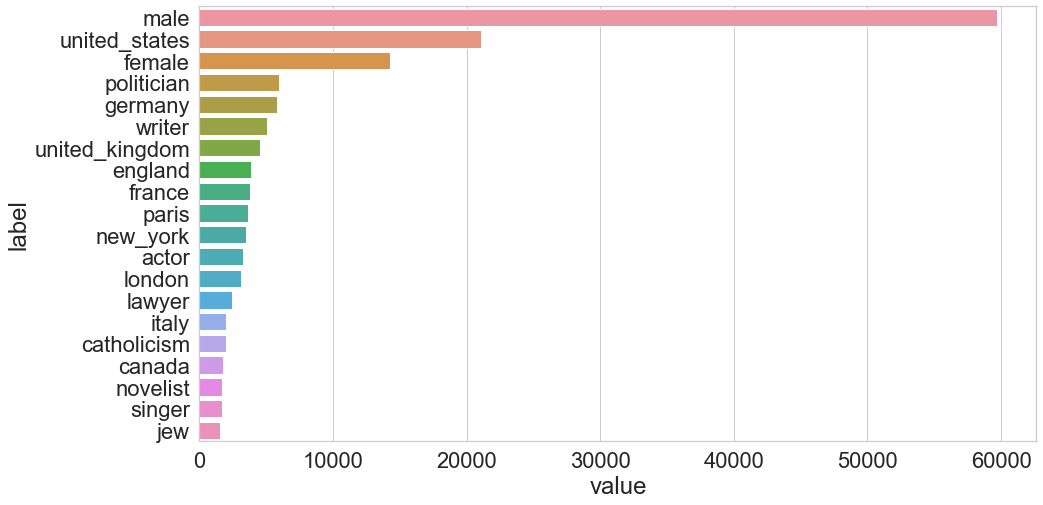
\includegraphics[width=1.0\linewidth, height=0.7\linewidth]{Freebase_Object_Counts}
		\captionsetup{justification=centering}
		\caption{Freebase}
	\end{subfigure}
	\captionsetup{justification=centering}
	\caption{KG object distribution. The number of times each subject takes part in a KG fact.}
\end{figure}

\begin{table}[H]
	\parbox{.5\linewidth}{
		\centering
		\begin{tabular}{lllllllllll}
  			\textbf{Statistic} & \textbf{Value}  \\
  			\hline
			Count & 33,011 \\
			Max & 537 \\
			Min & 1 \\
  			Median & 3 \\
  			IQR & 2 \\
				&
		\end{tabular}
		\caption{WordNet object statistics.}
		}
	\hfill
	\parbox{.5\linewidth}{
		\centering
		\begin{tabular}{lllllllllll}
  			\textbf{Statistic} & \textbf{Value}  \\
  			\hline
			Count & 15,342 \\
			Max & 59,663 \\
			Min & 1 \\
  			Median & 3 \\
  			IQR & 6 \\
				&
		\end{tabular}
		\caption{Freebase object statistics.}
		}
\end{table}

\noindent For WordNet, it can be seen that predicates are skewed toward "has instance" with $ 43, 312 $ occurrences, and "type of" with $ 36, 659 $ occurrences. Freebase predicates are somewhat more uniform, however four predicates have occurrences under $ 10, 000 $. \par

\noindent WordNet and Freebase subjects are somewhat uniform, although the median number of occurrences is 2 and 5 respectively, with an interquartile range (IQR) of $ 2 $ and $ 4 $ respectively, making these sparse distributions. WordNet object occurrences are somewhat uniform while Freebase object occurrences are skewed, with a single object, "male" occurring $ 59, 663 $ times, representing $15, 88\% $ of facts. This is in comparison to a median object occurrence of $ 3 $ and an IQR of $ 6 $. \par

\noindent The WordNet dataset is split into a training, validation and test set of $ 110, 362 \; (80.786 \%) $, $ 5, 215 \; (3.817 \%) $ and $ 21, 034 \; (15.397 \%) $ triples respectively.\ And the Freebase dataset is split into a training, validation and test set of $ 316, 232 \; (84.216 \%) $, $ 11, 815 \; (3.146 \%) $ and $ 47, 452 \; (12.637 \%) $ triples respectively. 


%********************************** %Optimised training algorithm **************************************

\subsection{Optimised training algorithm}

\noindent We update the NTN training algorithm to make of use of early stopping \unskip ~\citep{prechelt1998early}, the adaptive moment estimation (Adam) Adam optimiser \citep{kingma2014adam}, and use random search for hyperparameter optimisation \citep{bergstra2012random}. The model was trained on a MacBook Pro 2015 with 8 cores, 16GB RAM, and 512GB SSD, and no GPU acceleration. We evaluate the model by ranking the accuracy scores of the predicted triples for the respective datasets. \par

\noindent \textbf{Code to reproduce.} In the interest of reproducibility, all code needed to train and test the models in this section can be found at the following links. \newline
Baseline: \url{https://github.com/xhosaBoy/recursive-neural-tensor-networks} \newline
Optimised NTN training algorithm: \url{https://github.com/xhosaBoy/deep-knowledge-modelling} \par

\noindent \textbf{Link training results.} The cost and accuracy results of NTN model trained using the original baseline training algorithm, compared to the optimised training algorithm are presented in Figures 4.8 and 4.9. as well as Table 4.9.\ All experiments were only able to complete a maximum of $ 12 $ epochs before overwhelming compute resources. The maximum epoch runs are presented in the aforementioned figures. \par

\bigskip

\begin{figure}[H]
	\begin{subfigure}[b]{.5\linewidth}
   		\centering
    		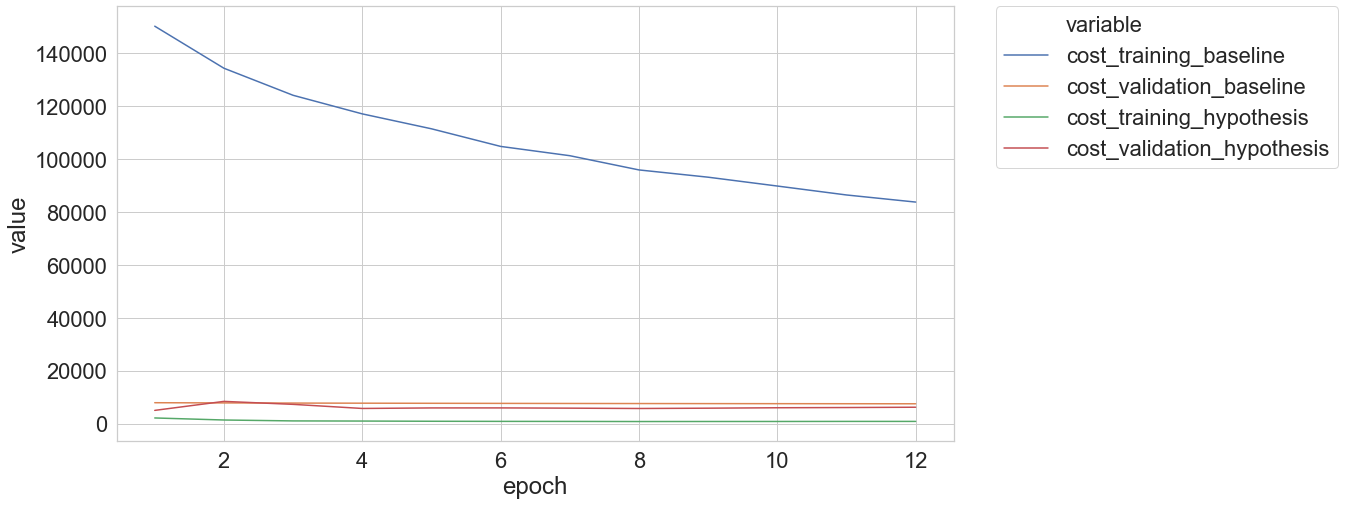
\includegraphics[width=1.0\linewidth, height=0.6\linewidth]{Wordnet_Cost_Results_Early_Stopping}
		\captionsetup{justification=centering}
		\caption{WordNet}
	\end{subfigure}
	\begin{subfigure}[b]{.5\linewidth}
   		\centering
		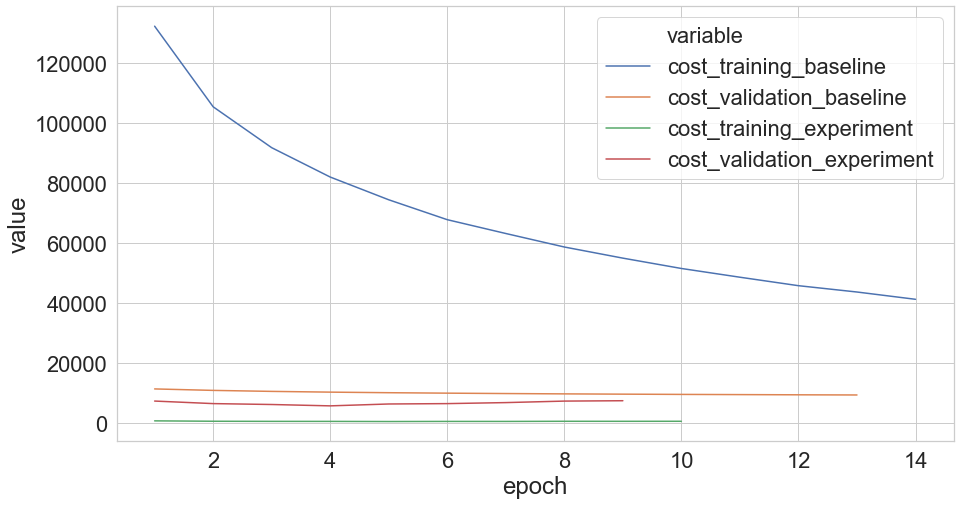
\includegraphics[width=1.0\linewidth, height=0.6\linewidth]{Freebase_Cost_Results}
		\captionsetup{justification=centering}
		\caption{Freebase}
	\end{subfigure}
	\captionsetup{justification=centering}
	\caption{Cost versus epoch for the respective KG. The training set cost for the baseline algorithm clearly descends as epochs increase. The training cost for the optimised (hypothesis) algorithm is almost identical to the validation cost after the first epoch, demonstrating the effectiveness of the updates. }
\end{figure}

\begin{figure}[H]
	\begin{subfigure}[b]{.5\linewidth}
   		\centering
    		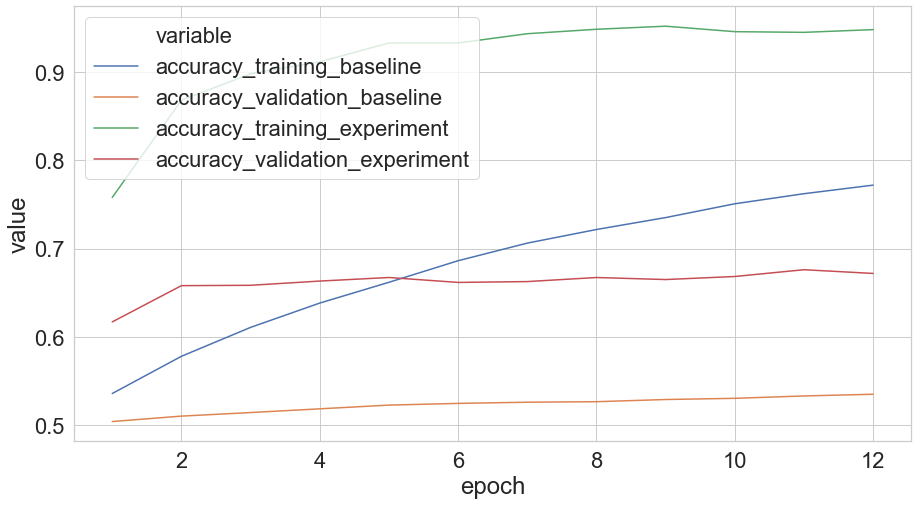
\includegraphics[width=1.0\linewidth, height=0.6\linewidth]{Wordnet_Accuracy_Results_Early_Stopping}
		\captionsetup{justification=centering}
		\caption{WordNet}
	\end{subfigure}
	\begin{subfigure}[b]{.5\linewidth}
   		\centering
		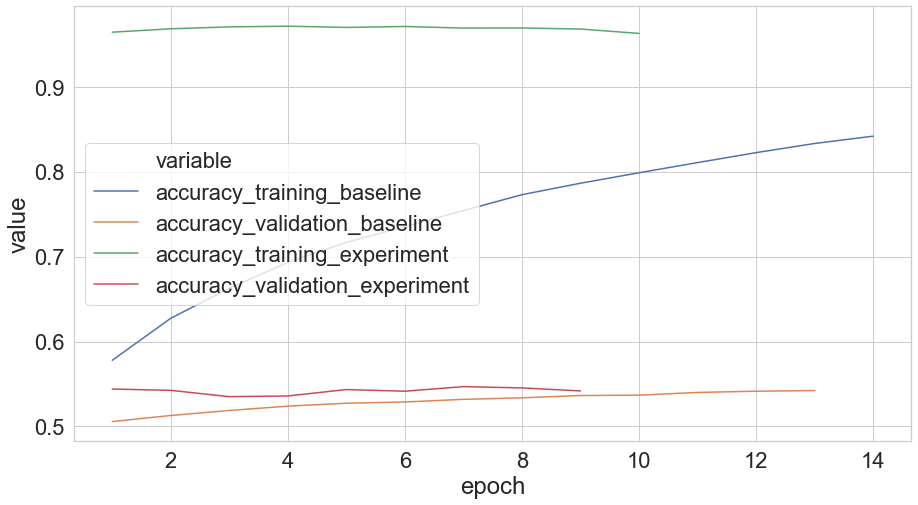
\includegraphics[width=1.0\linewidth, height=0.6\linewidth]{Freebase_Accuracy_Results}
		\captionsetup{justification=centering}
		\caption{Freebase}
	\end{subfigure}
	\captionsetup{justification=centering}
	\caption{Accuracy versus epoch for the respective KG. The optimised algorithm accuracy is significantly higher than the baseline algorithm. Once again demonstrating the effectiveness of the updates.}
\end{figure}

\begin{table}[H]
	\centering
	\begin{tabular}{lllllllllll}
  		\textbf{Model} & \textbf{WordNet} & \textbf{Freebase} & \textbf{Avg} \\
  		\hline
  		Distance Model \unskip ~\citep{bordes2011learning} & .683 & .610 & .647 \\
  		Original NTN \unskip ~\citep{socher2013reasoning} & \textbf{.862} & \textbf{.90} & \textbf{.881} \\
  		Reimplimented NTN Baseline  \unskip ~\citep{Doss2015} & .562 & .535 & .549 \\
  		\hline
  		Optimised NTN (Ours) & .674 & .548 & .611 \\
		&
	\end{tabular}
	\captionsetup{justification=centering}
	\caption{Cost and accuracy on WordNet and Freebase KG test sets. Our reimplimented NTN with optimised training algorithm out performs the baseline NTN across both cost and accuracy measurements. The original NTN algorithm however significantly outperforms all models. This may be due to differences other training algorithm properties such as number of epochs, batch size, and hyperparameter values.}
\end{table}


%********************************** %HypER and Covariate Shift  **************************************

\section{HypER and HypER+}

\subsection{Baseline training algorithm}
\textbf{Model summary.} HypER is a model that takes the convolution between a predicate-specific filter and subject vector, generating a subject-predicate feature map. This map is flattened and passed through a nonlinearity, before an inner product is taken with an object vector. The result is a relational score which is passed through a logistic sigmoid to generate a probability of a potential relationship between the two entities. \par

\noindent \textbf{Binary cross-entropy loss.} The binary cross-entropy loss is used to train HypER. Like the NTN model, the input consists of a subject-predicate pair, and an object is presented as a target to complete the triple. A relational score is generated for each sample and passed through a logistic sigmoid. Loss is generated by comparing the produced likelihood with the expected likelihood, $ 0 $ or $ 1 $. The sum of losses in a batch of samples is aggregated and backpropagated through the network for parameter update. \par

\noindent \textbf{Benchmark metrics.} The current suite of link prediction benchmark metrics includes Hit@10, Hit@3, Hit@1, Mean Rank, and Mean Reciprocal Rank.\ For these models, all objects in the KG are assigned a probability and then ranked in descending order. The Hit@X metrics comprise the relation prediction accuracy measures of the model, where X describes the lowest rank the predicted object can occupy. For example in Hit@10, only the top 10 objects are considered as accurate. The Mean Rank is the average predicted object rank for Hit@1 after each epoch, for example a Mean Rank of 100 after epoch 1, and Mean rank of 50 after 10 epoch. The Mean Reciprocal Rank is the inverse of the Mean rank. \par

\noindent \textbf{Experimental setup.} We use the following two link prediction benchmark datasets. WN18 \citep{bordes2013translating} is a subset of WordNet, a database containing lexical relations between words. It contains $ 40, 943 $ entities and $ 18 $ relations. FB15k \citep{bordes2013translating} is a subset of Freebase, a large database of facts about the real world. FB15k contains $ 14, 951 $ entities and $ 1, 345 $ relations. Visualisations of the respective KGs, as well as a sample of RDF triple encoded facts, are presented in Figures 4.10 to 4.13.\ Property counts for the respective KGs are presented in Tables 4.10 and 4.11. \par

\bigskip

\begin{figure}[H]
   	\centering
    	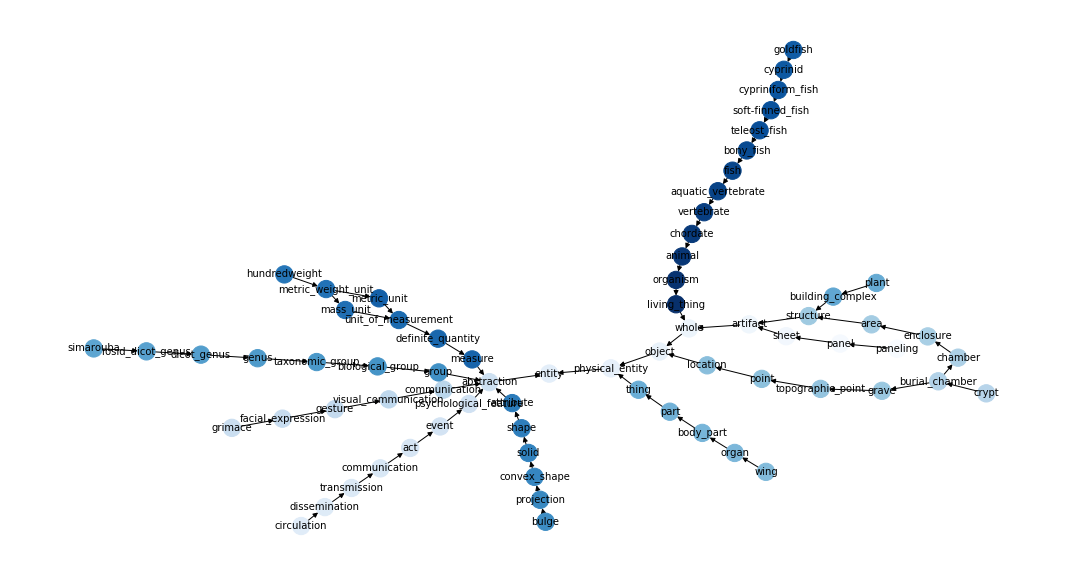
\includegraphics[width=0.9\textwidth, height=0.5\textwidth]{WN18_Graph}
	\captionsetup{justification=centering}
	\caption{A subset of WN18 facts structured as a KG. Entities are nodes, and relations are edges, where a fact is encoded as an RDF triple.}
\end{figure}

\begin{figure}[H]
   	\centering
    	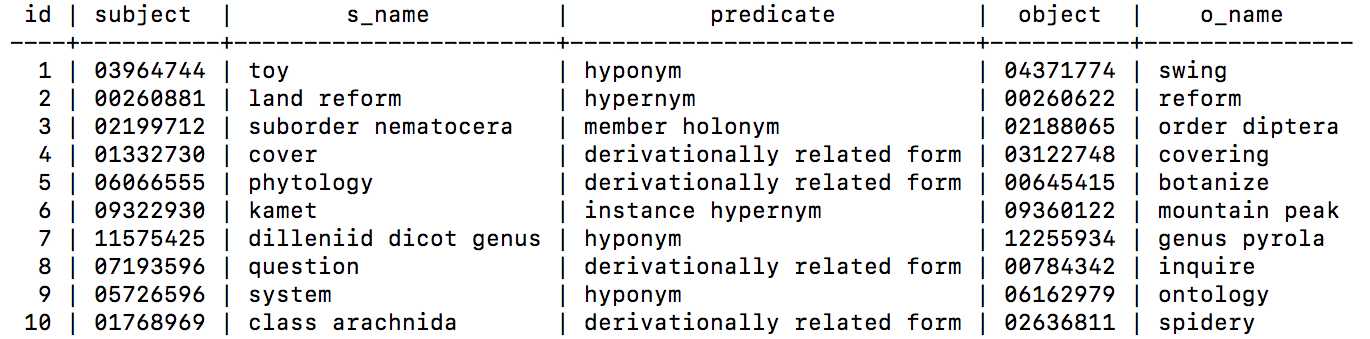
\includegraphics[width=0.9\textwidth, height=0.3\textwidth]{wn18_fact_sample}
	\captionsetup{justification=centering}
	\caption{A sample of RDF triples from the WN18 KG.}
\end{figure}

\begin{figure}[H]
   	\centering
    	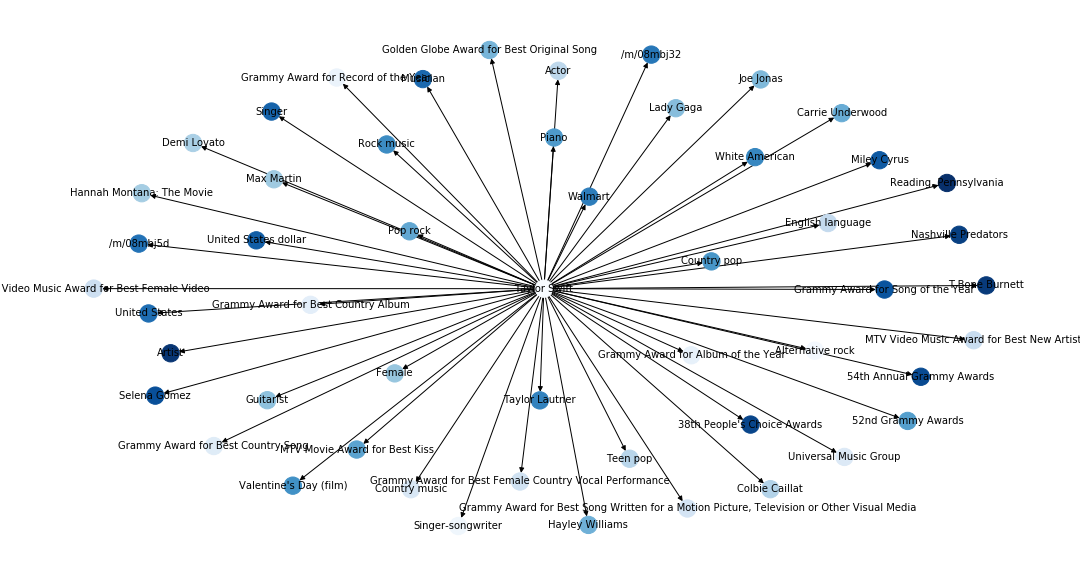
\includegraphics[width=0.9\textwidth, height=0.5\textwidth]{FB15k_Graph}
	\captionsetup{justification=centering}
	\caption{A subset of FB15k facts structured as a KG. Entities are nodes, and relations are edges, where a fact is encoded as an RDF triple.}
\end{figure}

\begin{figure}[H]
   	\centering
    	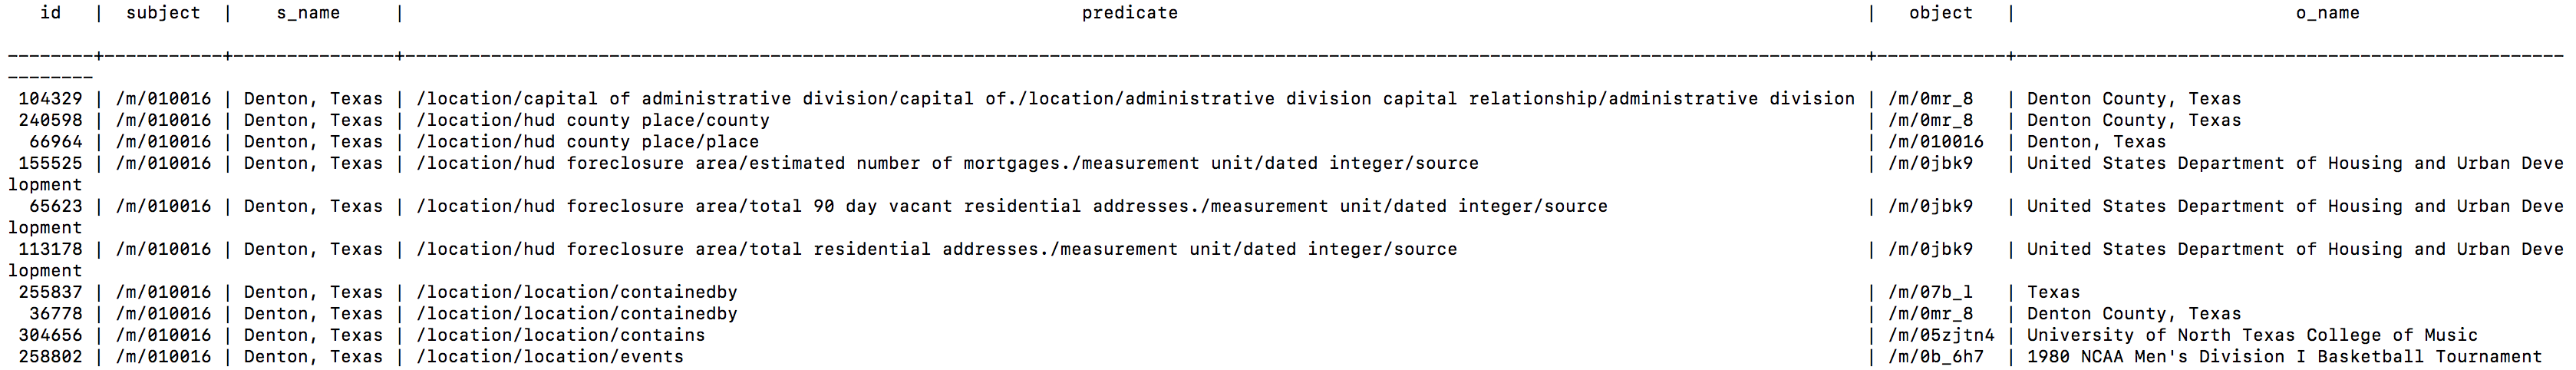
\includegraphics[width=1.0\textwidth, height=0.3\textwidth]{fb15k_fact_sample}
	\captionsetup{justification=centering}
	\caption{A sample of RDF triples from the FB15k KG.}
\end{figure}

\noindent Here we used the PyTorch framework to develop our model. This model is built on top of the HypER model introduced by Bala\u{z}ev\'{i}c et al. \unskip ~\citep{balazevic2019hypernetwork}. Random entity and relational embeddings are used to initialise model training. These embeddings are dynamically adjusted during the training process to generate latent representations specific to the KG.

\bigskip

\begin{table}[H]
	\parbox{.5\linewidth}{
		\centering
		\begin{tabular}{lllllllllll}
  			\textbf{Property} & \textbf{Count}  \\
  			\hline
  			subjects & 40,943  \\
  			predicates & 18  \\
  			triples & 151,442 \\
			&
		\end{tabular}
		\captionsetup{justification=centering}
		\caption{Counts of WN18 KG elements.}
		}
	\hfill
	\parbox{.5\linewidth}{
		\centering
		\begin{tabular}{lllllllllll}
  			\textbf{Property} & \textbf{Count}  \\
  			\hline
  			subjects & 14,951   \\
  			predicates & 1,345  \\
  			triples & 592,213  \\
			&
		\end{tabular}
		\captionsetup{justification=centering}
		\caption{Counts of FB15k KG elements.}
		}
\end{table}


%********************************** %Predicate  **************************************

\noindent Summary statistics of the respective KG RDF formalism are presented in Figures 4.14 to 4.16, and Tables 4.12 and 4.17. 

\begin{figure}[H]
   	\centering
    	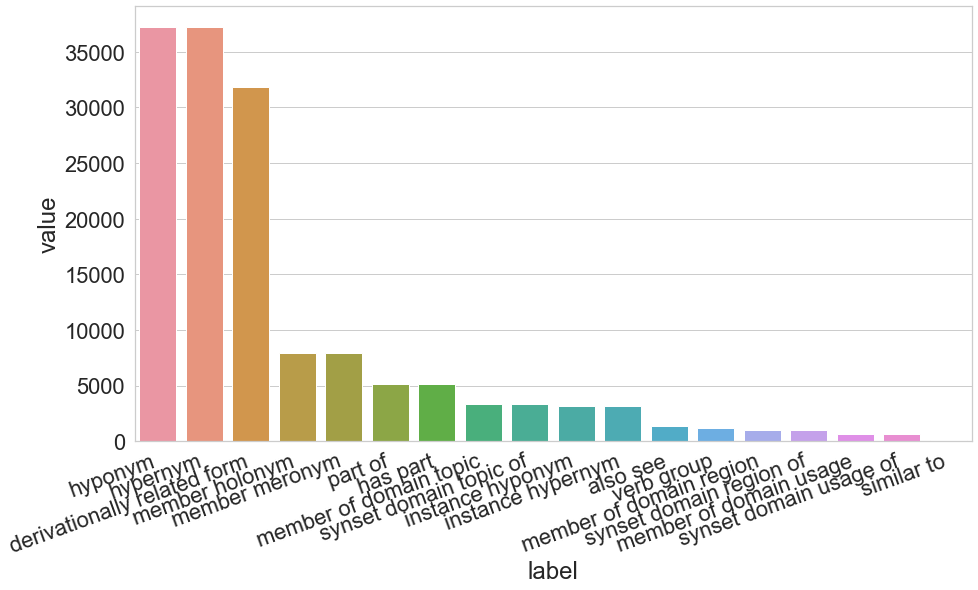
\includegraphics[width=0.7\textwidth, height=0.3\textheight]{WN18_Predicate_Counts}
	\captionsetup{justification=centering}
	\caption{WN18 predicate distribution in KG facts.}
\end{figure}

\begin{table}[H]
		\centering
		\begin{tabular}{lllllllllll}
  			\textbf{Statistic} & \textbf{Value}  \\
  			\hline
			Count & 18 \\
			Max & 37,221  \\
			Min & 86 \\
  			Median & 3,242.5  \\
  			IQR & 6,190.75  \\
			&
		\end{tabular}
		\caption{WN18 predicate statistics.}
\end{table}

\begin{figure}[H]
   	\centering
    	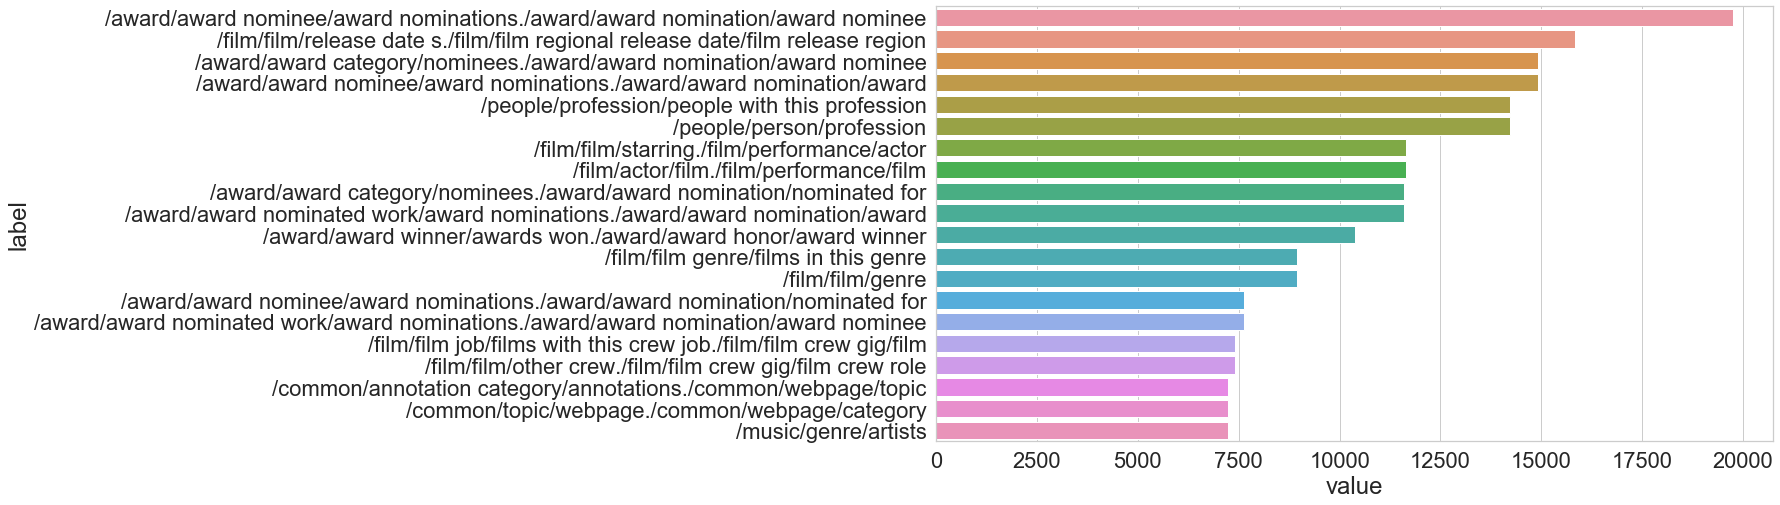
\includegraphics[width=1.0\textwidth, height=0.3\textheight]{FB15k_Predicate_Counts}
	\captionsetup{justification=centering}
	\caption{FB15k predicate distribution in KG facts.}
\end{figure}

\begin{table}[H]
		\centering
		\begin{tabular}{lllllllllll}
  			\textbf{Statistic} & \textbf{Value}  \\
  			\hline
			Count & 1,345 \\
			Max & 19,764  \\
			Min & 1  \\
  			Median & 26  \\
  			IQR & 166  \\
			&
		\end{tabular}
		\caption{FB15k predicate statistics.}
\end{table}

%********************************** %Subject **************************************

\begin{figure}[H]
	\begin{subfigure}[b]{.5\linewidth}
   		\centering
    		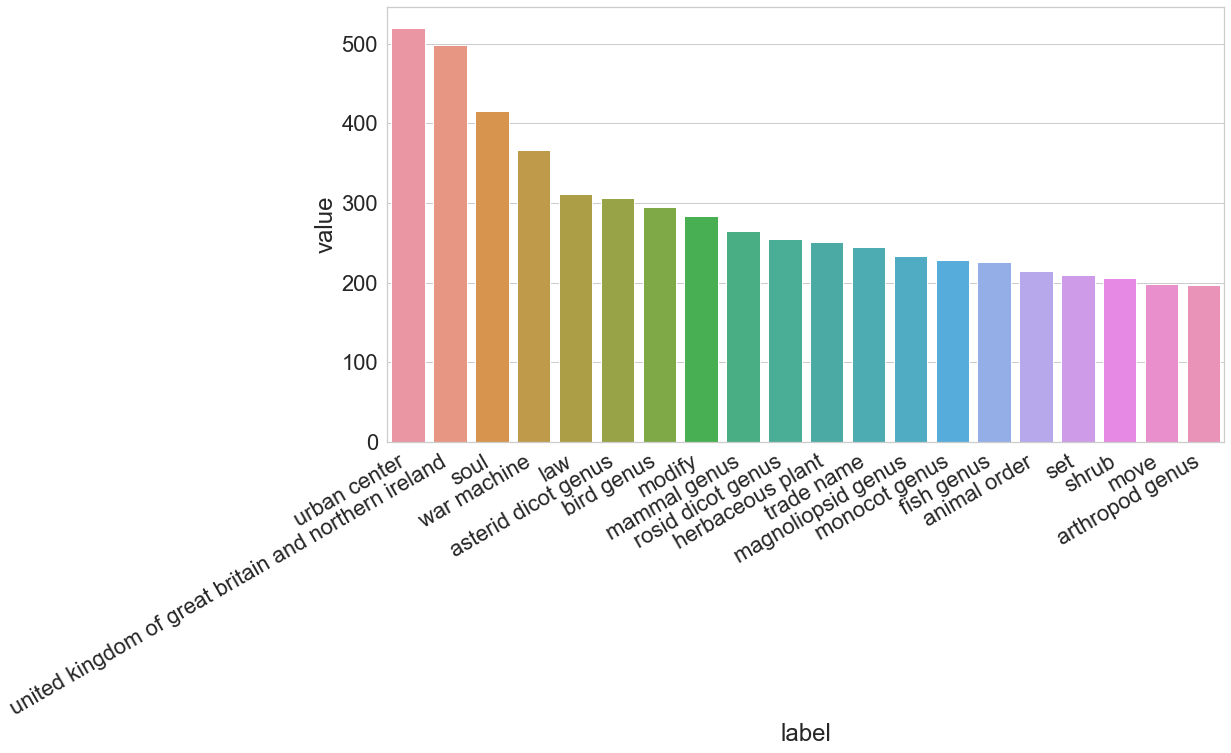
\includegraphics[width=1.0\linewidth, height=0.7\linewidth]{WN18_Subject_Counts}
		\captionsetup{justification=centering}
		\caption{WN18}
	\end{subfigure}
	\begin{subfigure}[b]{.5\linewidth}
   		\centering
		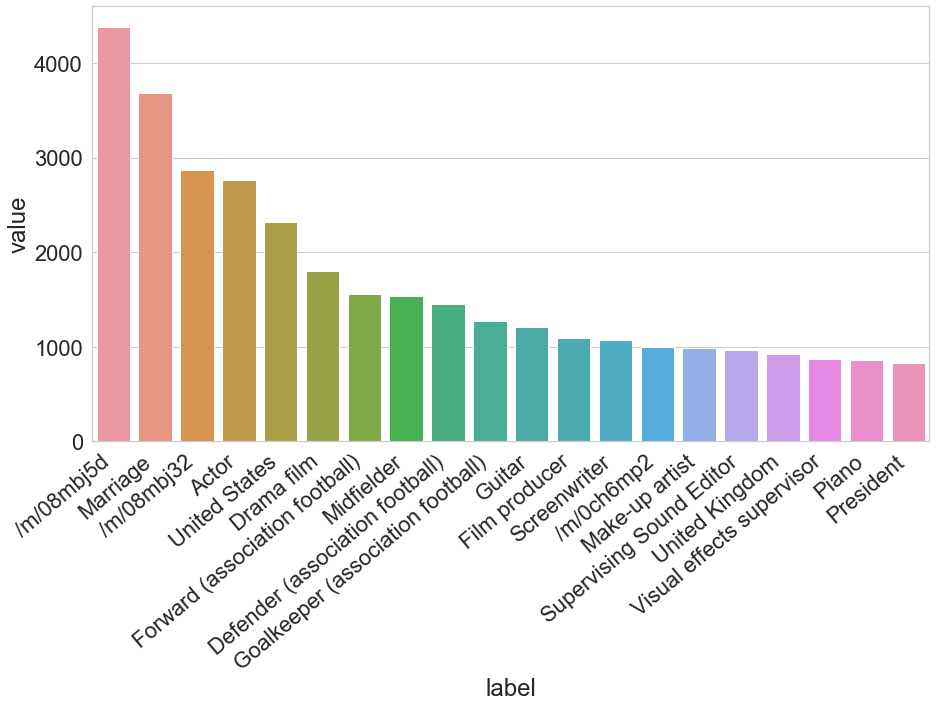
\includegraphics[width=1.0\linewidth, height=0.7\linewidth]{FB15k_Subject_Counts}
		\captionsetup{justification=centering}
		\caption{FB15k}
	\end{subfigure}
	\captionsetup{justification=centering}
	\caption{KG subject distribution. The number of times each subject takes part in a KG fact.}
\end{figure}

\begin{table}[H]
	\parbox{.5\linewidth}{
		\centering
		\begin{tabular}{lllllllllll}
  			\textbf{Statistic} & \textbf{Value}  \\
  			\hline
			Count & 32,544 \\
			Max & 520 \\
			Min & 1 \\
  			Median & 3 \\
  			IQR & 2 \\
			&
		\end{tabular}
		\caption{WN18 subject statistics.}
		}
	\hfill
	\parbox{.5\linewidth}{
		\centering
		\begin{tabular}{lllllllllll}
  			\textbf{Statistic} & \textbf{Value}  \\
  			\hline
			Count &14,865 \\
			Max & 4,381 \\
			Min & 1 \\
  			Median & 27 \\
  			IQR & 32 \\
			&
		\end{tabular}
		\caption{FB15k subject statistics.}
		}
\end{table}

%********************************** %Object  **************************************

\begin{figure}[H]
	\begin{subfigure}[b]{.5\linewidth}
   		\centering
    		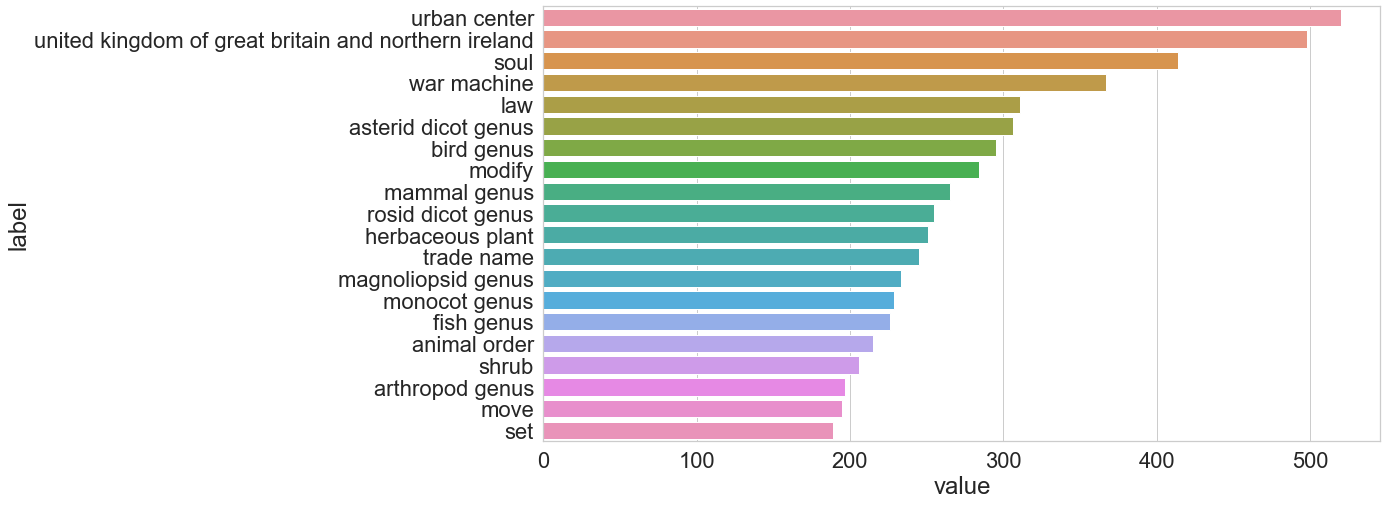
\includegraphics[width=1.0\linewidth, height=0.7\linewidth]{WN18_Object_Counts}
		\captionsetup{justification=centering}
		\caption{WN18}
	\end{subfigure}
	\begin{subfigure}[b]{.5\linewidth}
   		\centering
		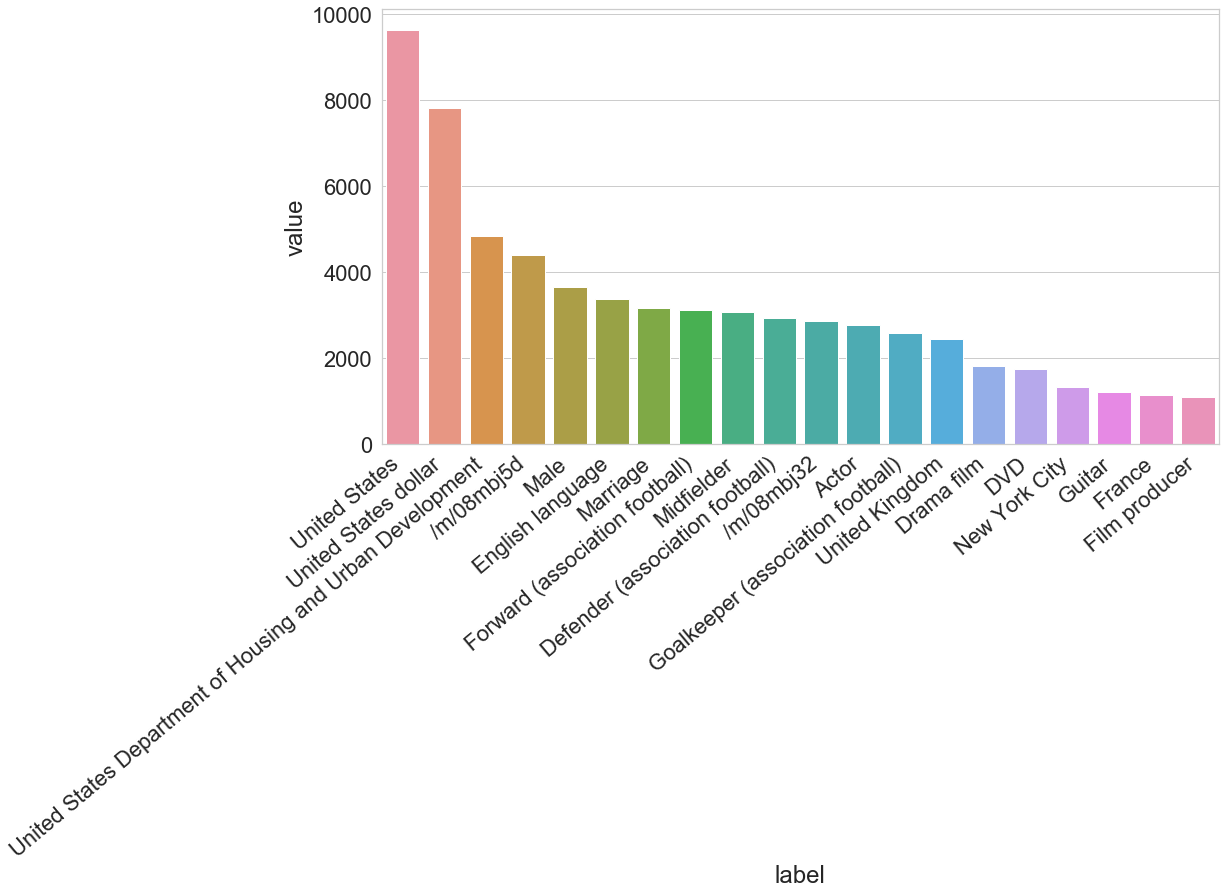
\includegraphics[width=1.0\linewidth, height=0.7\linewidth]{FB15k_Object_Counts}
		\captionsetup{justification=centering}
		\caption{FB15k}
	\end{subfigure}
	\captionsetup{justification=centering}
	\caption{KG object distribution. The number of times each subject takes part in a KG fact.}
\end{figure}

\begin{table}[H]
	\parbox{.5\linewidth}{
		\centering
		\begin{tabular}{lllllllllll}
  			\textbf{Statistic} & \textbf{Value}  \\
  			\hline
			Count & 32,543 \\
			Max & 520 \\
			Min & 1 \\
  			Median & 3 \\
  			IQR & 2 \\
			&
		\end{tabular}
		\caption{WN18 object statistics.}
		}
	\hfill
	\parbox{.5\linewidth}{
		\centering
		\begin{tabular}{lllllllllll}
  			\textbf{Statistic} & \textbf{Value}  \\
  			\hline
			Count & 14,930 \\
			Max & 9,645 \\
			Min & 1 \\
  			Median & 23 \\
  			IQR & 30 \\
			&
		\end{tabular}
		\caption{FB15k object statistics.}
		}
\end{table}

\noindent For WN18, it can be seen that predicates are skewed toward the relations "hyponym",  "hypernym", and "derivationally related from", with a maximum of $ 37, 221 $ occurrences. FB15k predicates are somewhat more uniform. \par

\noindent WN18 and FB15k subjects are somewhat uniform aside from a small number of high occurring entities, with the median number of occurrences being $ 3 $ and $ 27 $ respectively, and with an IQR of $ 2 $ and $ 32 $ respectively. WN18 object occurrences are somewhat uniform. FB15k object occurrences are skewed, with the "United States" partaking in the highest number of triples. This is in comparison to a median object occurrence of $ 23 $ and an IQR of 30. \par

\noindent The WN18 dataset is split into a training, validation and test set of $ 141, 442 \; (93.397 \%) $, $ 5, 000 \; (3.302 \%) $ and $ 5, 000 \; (3.302 \%) $ triples respectively.\ And the FB15k dataset is split into a training, validation and test set of $ 483, 142 \; (81.582 \%) $, $ 50, 000 \; (8.443 \%) $ and $ 59, 071 \; (9.975 \%) $ triples respectively. 


%********************************** %HypER+  **************************************

\subsection{HypER+}
HypER predicate filter inputs generated by a hypernetwork may suffer from distribution shift during training. We compensate for this covariate shift by introducing batch normalisation for predicate inputs, and call this model HypER+. The model was trained on Google Cloud Platform, on an N1 series instance with  8 CPU cores, 30GB RAM, 512GB SSD and an Nvidia Tesla P100 GPU. We train the respective models for $ 500 $ epoch, and evaluate them using the standard link prediction benchmarks discussed earlier. \par

\noindent \textbf{Code to reproduce.} In the interest of reproducibility, all code needed to train and test the models in this section can be found at the following links. \newline
Baseline: \url{https://github.com/xhosaBoy/HypER-baseline} \newline
HypER+: \url{https://github.com/xhosaBoy/HypER-Regularised-Relations} \par

\noindent \textbf{Link prediction results.} The cost and suite of current standard link prediction benchmark metrics, including Hit@10, Hit@3, Hit@1, Mean Rank and Mean Reciprocal Rank, results of the HypER+ model, compared against the HypER model baseline, are presented in Figures 4.18 and 4.23. as well as Tables 4.18 and 4.19. \par


%********************************** %Cost  **************************************

\bigskip

\begin{figure}[H]
	\begin{subfigure}[b]{.5\linewidth}
   		\centering
    		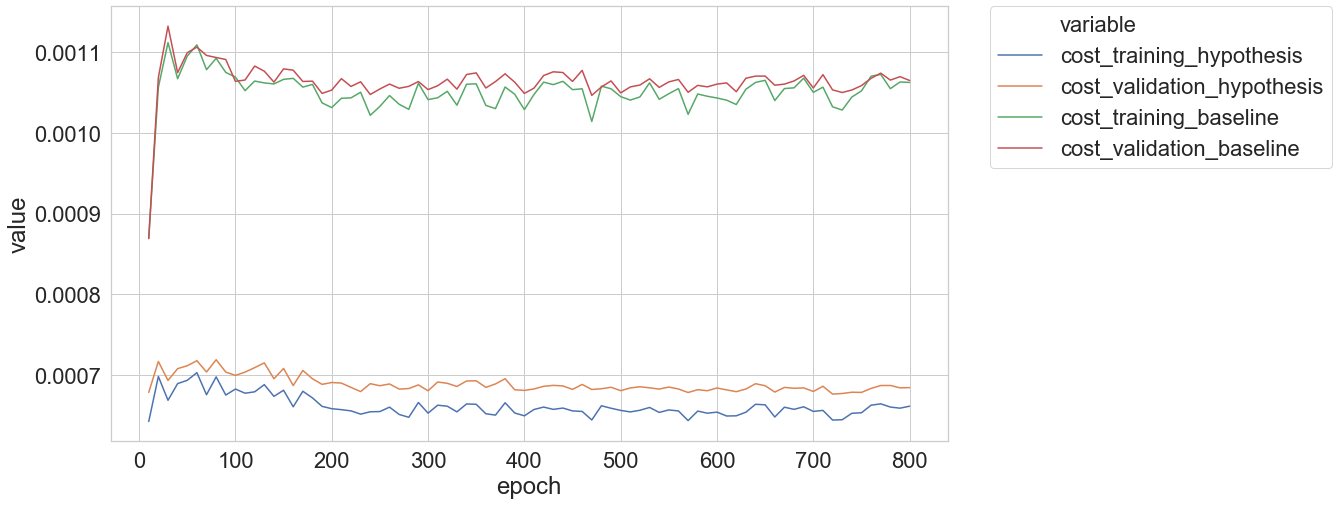
\includegraphics[width=1.0\linewidth, height=0.6\linewidth]{WN18_Cost_Results}
		\captionsetup{justification=centering}
		\caption{WN18}
	\end{subfigure}
	\begin{subfigure}[b]{.5\linewidth}
   		\centering
		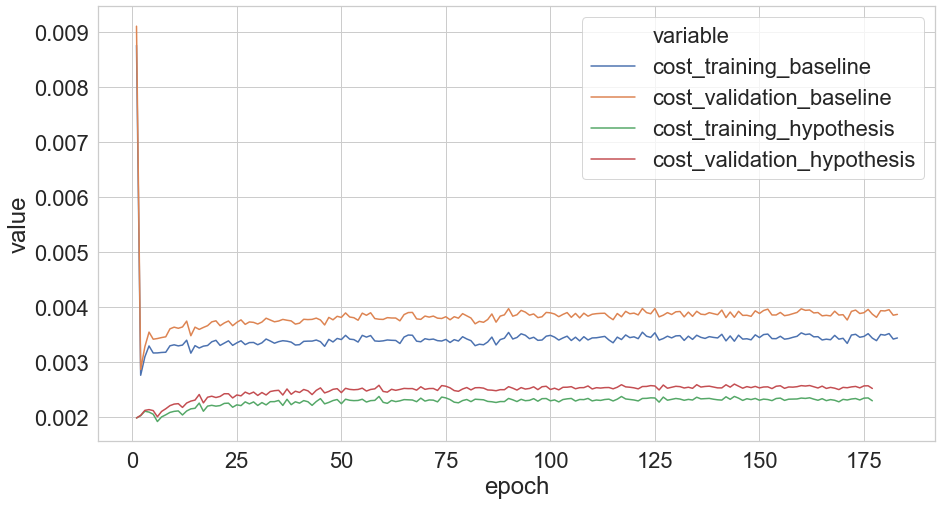
\includegraphics[width=1.0\linewidth, height=0.6\linewidth]{FB15k_Cost_Results}
		\captionsetup{justification=centering}
		\caption{FB15k}
	\end{subfigure}
	\captionsetup{justification=centering}
	\caption{Cost versus epoch for the respective KG. There is a large difference between the HypER (baseline) and HypER+ (hypothesis) costs, where the hypothesis outperforms the baseline on both KGs by quite some margin. The FB15k costs exhibit strange behaviour, dropping sharply in the first 10 epochs, before rising and plateauing. This could be attributed to small probabilities first computed by the models, before becoming more confident with larger probabilities. The FB15k cost is also higher than the WN18 cost, this may be due their respective KG size and complexity.}
\end{figure}

%********************************** %Hits@10  **************************************

\begin{figure}[H]
	\begin{subfigure}[b]{.5\linewidth}
   		\centering
    		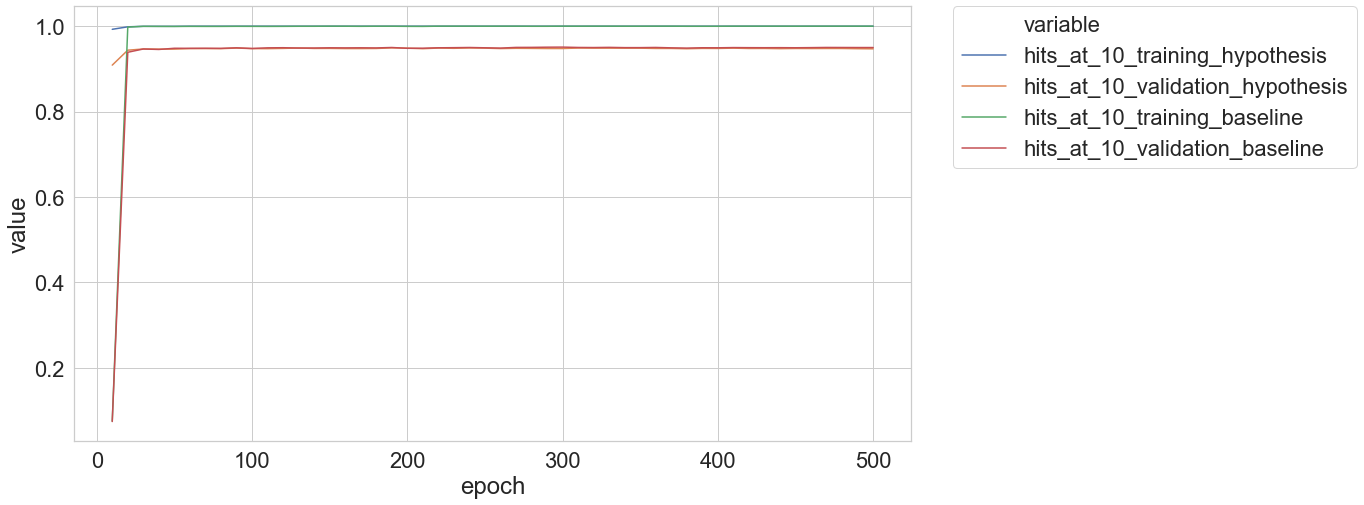
\includegraphics[width=1.0\linewidth, height=0.6\linewidth]{WN18_hits_at_10_Results}
		\captionsetup{justification=centering}
		\caption{WN18}
	\end{subfigure}
	\begin{subfigure}[b]{.5\linewidth}
   		\centering
		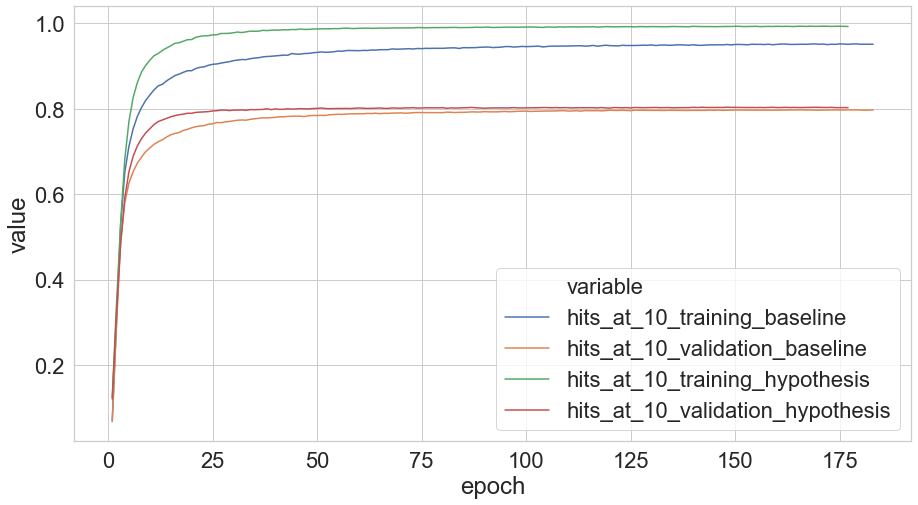
\includegraphics[width=1.0\linewidth, height=0.6\linewidth]{FB15k_hits_at_10_Results}
		\captionsetup{justification=centering}
		\caption{FB15k}
	\end{subfigure}
	\captionsetup{justification=centering}
	\caption{Hits@10 versus epoch for the respective KG. There is hardly any difference between the hypothesis and baseline models for the WN18 KG. The hypothesis model once again outperforms the baseline on the FB15k KG, although the validation difference is not as pronounced as the training difference. Once again the WN18 KG has higher performance, and both metrics reach a plateau.}
\end{figure}

%********************************** %Hits@3  **************************************

\begin{figure}[H]
	\begin{subfigure}[b]{.5\linewidth}
   		\centering
    		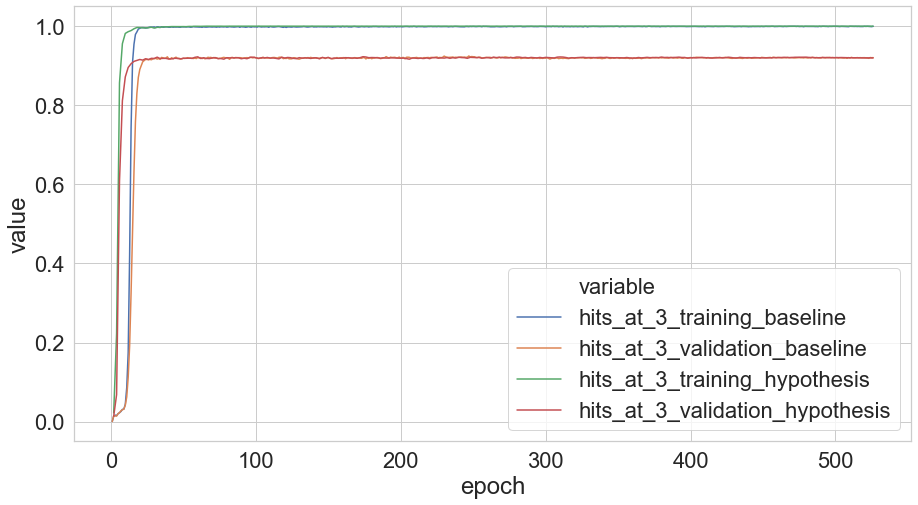
\includegraphics[width=1.0\linewidth, height=0.6\linewidth]{WN18_hits_at_3_Results}
		\captionsetup{justification=centering}
		\caption{WN18}
	\end{subfigure}
	\begin{subfigure}[b]{.5\linewidth}
   		\centering
		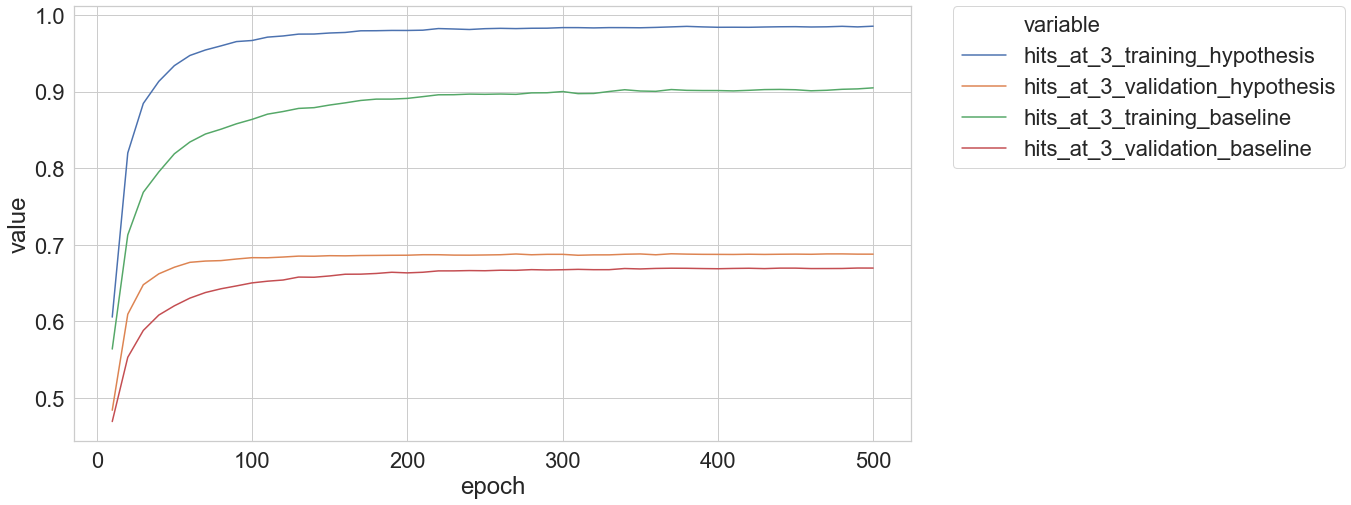
\includegraphics[width=1.0\linewidth, height=0.6\linewidth]{FB15k_hits_at_3_Results}
		\captionsetup{justification=centering}
		\caption{FB15k}
	\end{subfigure}
	\captionsetup{justification=centering}
	\caption{Hits@3 versus epoch for the respective KG. The models have similar behaviour to the Hit@10 metric, and both have lower accuracy. There is however a larger performance difference between the hypothesis and baseline. This may be due to the more robust generalisation requirements with a smaller subset of acceptable answers, Hit@3 vs Hit@10, resulting in a more pronounced impact from covariate shift of predicate latent parameters.}
\end{figure}

%********************************** %Hits@1  **************************************

\begin{figure}[H]
	\begin{subfigure}[b]{.5\linewidth}
   		\centering
    		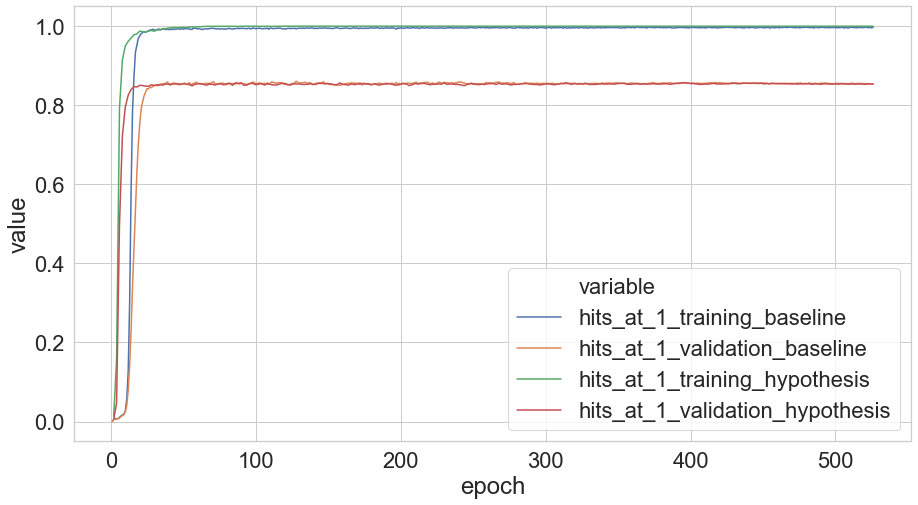
\includegraphics[width=1.0\linewidth, height=0.6\linewidth]{WN18_hits_at_1_Results}
		\captionsetup{justification=centering}
		\caption{WN18}
	\end{subfigure}
	\begin{subfigure}[b]{.5\linewidth}
   		\centering
		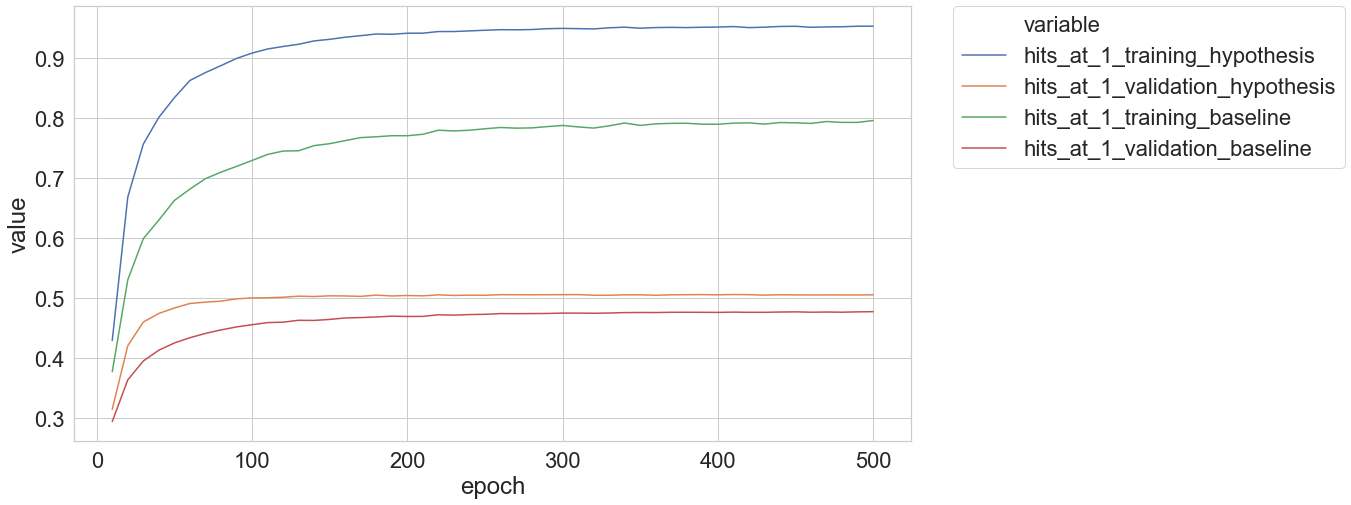
\includegraphics[width=1.0\linewidth, height=0.6\linewidth]{FB15k_hits_at_1_Results}
		\captionsetup{justification=centering}
		\caption{FB15k}
	\end{subfigure}
	\captionsetup{justification=centering}
	\caption{Hits@1 versus epoch for the respective KG. Once more the models have similar behaviour to the Hit@10 and Hit@3 metrics, and both have even lower accuracy. There is no discernible difference between the models on the WN18 KG, however there is once again a larger difference between them on the FB15k KG. }
\end{figure}

%********************************** %Mean rank **************************************

\begin{figure}[H]
	\begin{subfigure}[b]{.5\linewidth}
   		\centering
    		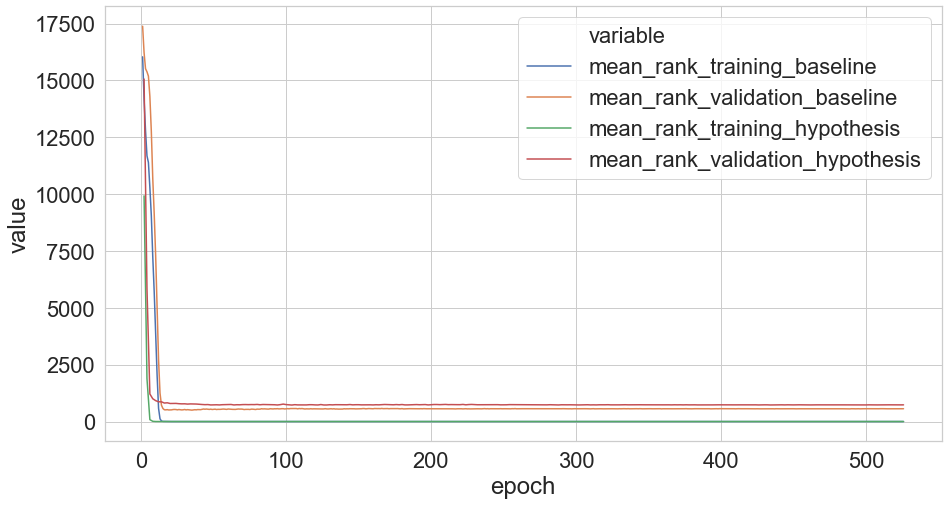
\includegraphics[width=1.0\linewidth, height=0.6\linewidth]{WN18_mean_rank_Results}
		\captionsetup{justification=centering}
		\caption{WN18}
	\end{subfigure}
	\begin{subfigure}[b]{.5\linewidth}
   		\centering
		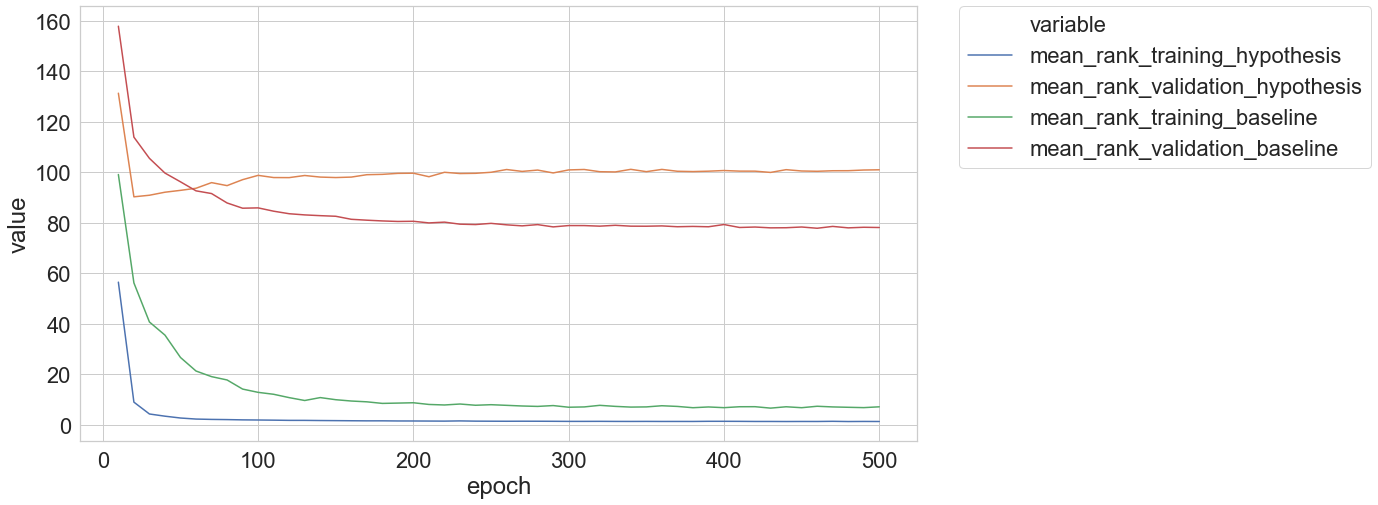
\includegraphics[width=1.0\linewidth, height=0.6\linewidth]{FB15k_mean_rank_Results}
		\captionsetup{justification=centering}
		\caption{FB15k}
	\end{subfigure}
	\captionsetup{justification=centering}
	\caption{Mean Rank versus epoch for the respective KG. Not surprisingly, the training set outperforms the validation set on mean rank. There is also now a discernible difference in performance on the WN18 KG. For the first time, the hypothesis outperformed by the baseline on both KGs. One potential reason for the this is that $ 50^{th} $ percentile accuracy of the baseline is higher, where as the hypothesis is more accurate at higher percentiles, e.g. $ 90^{th} $.}
\end{figure}

%********************************** %Mean reciprocal rank **************************************

\begin{figure}[H]
	\begin{subfigure}[b]{.5\linewidth}
   		\centering
    		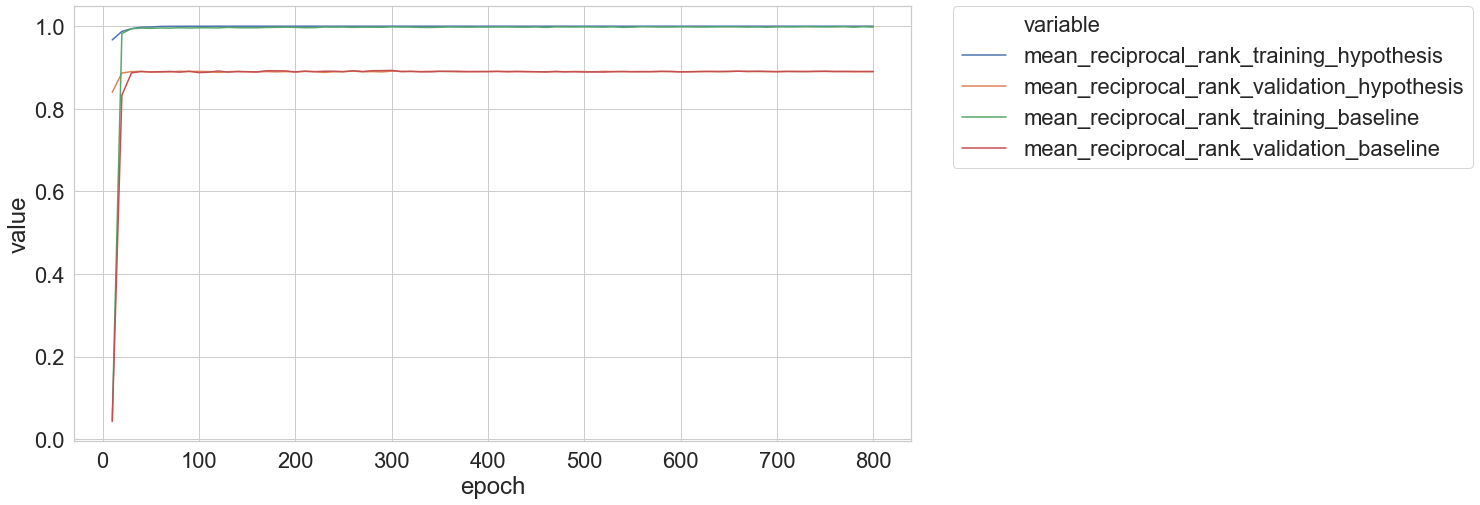
\includegraphics[width=1.0\linewidth, height=0.6\linewidth]{WN18_mean_reciprocal_rank_Results}
		\captionsetup{justification=centering}
		\caption{WN18}
	\end{subfigure}
	\begin{subfigure}[b]{.5\linewidth}
   		\centering
		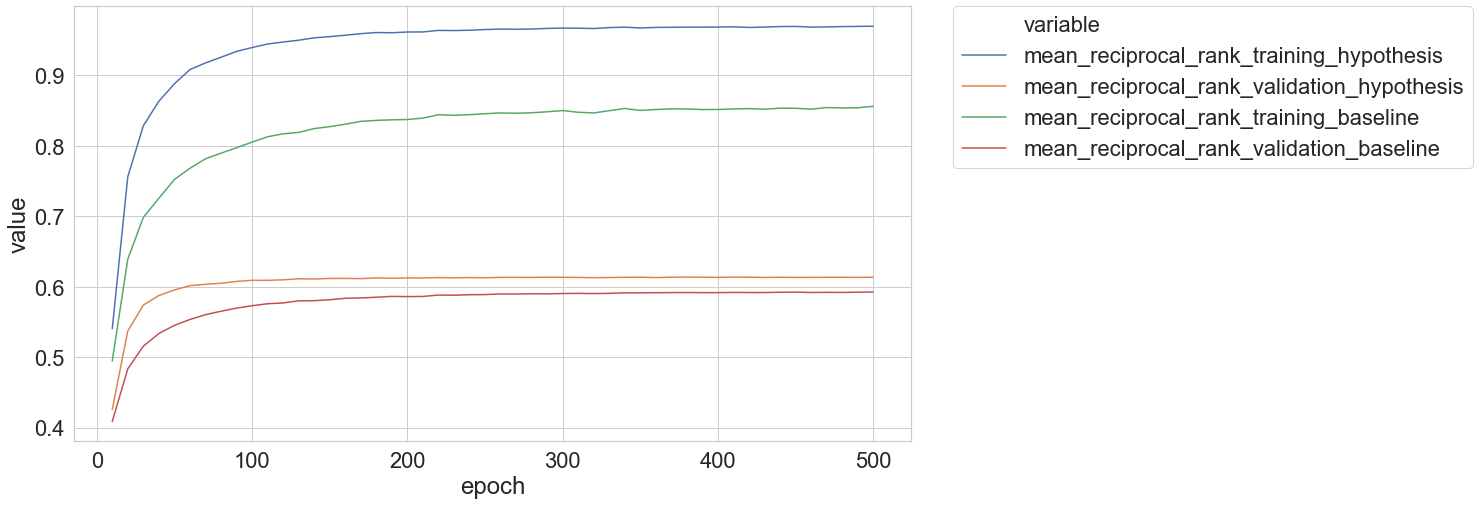
\includegraphics[width=1.0\linewidth, height=0.6\linewidth]{FB15k_mean_reciprocal_rank_Results}
		\captionsetup{justification=centering}
		\caption{FB15k}
	\end{subfigure}
	\captionsetup{justification=centering}
	\caption{Mean Reciprocal Rank versus epoch for the respective KG. There is no discernible difference in performance on the WN18 KG, however the hypothesis is once again outperforms the baseline on the FB15k KG.}
\end{figure}

%********************************** %Test results **************************************

\begin{table}[H]
		\centering
		\begin{tabular}{lllllllllll}
  			\textbf{Model} & \textbf{H@10} & \textbf{H@3} & \textbf{H@1} & \textbf{MR} & \textbf{MRR} \\
  			\hline
  			TransE \unskip~\citep{bordes2013translating} & .892 & - & - & \textbf{251} & - \\
  			DistMult \unskip~\citep{yang2014embedding} & .936 & .914 & .728 & 902 & .822 \\
  			ComplEx \unskip~\citep{trouillon2016complex} & .947 & .936 & .936 & - & .941 \\
  			Neural LP \unskip~\citep{yang2017differentiable} & .945 & - & - & - & .940 \\
			R-GCN \unskip~\citep{schlichtkrull2018modeling}) & \textbf{.964} & .929 & .697 & - & .819 \\
			TorusE \unskip~\citep{ebisu2018toruse} & .954 & .950 & .943 & - & .947 \\
			ConvE \unskip~\citep{dettmers2018convolutional} & .956 & .946 & .935 & 374 & .943 \\
			HypER \unskip~\citep{balazevic2019hypernetwork} & .958 & \textbf{.955} & \textbf{.947} & 431 & \textbf{.951} \\
  			\hline
  			HypER+ (ours) & .957 & .954 & .946 & 565 & .950 \\
			&
		\end{tabular}
		\captionsetup{justification=centering}
		\caption{Relation prediction test results on WN18. The hypothesis is outperformed by the baseline across all metrics. It should however be noted that the difference is in the order of a $ 0.1\% $, indicating almost identical performance. This is consistent with training and validation results discussed earlier. Interestingly the R-GCN model achieves the highest Hit@10 performance. This model uses the graph modelling SRL paradigm, as opposed to latent feature modelling, it however performs poorly across all other metrics. There may however be opportunity in exploring this paradigm further. }
\end{table}

\begin{table}[H]
		\centering
		\begin{tabular}{lllllllllll}
  			\textbf{Model} & \textbf{H@10} & \textbf{H@3} & \textbf{H@1} & \textbf{MR} & \textbf{MRR} \\
  			\hline
  			TransE \unskip~\citep{bordes2013translating} & .471 & - & - & 125 & - \\
  			DistMult (\unskip~\citep{yang2014embedding} & .824 & .733 & .546 & 97 & .654 \\
  			ComplEx \unskip~\citep{trouillon2016complex} & .840 & .759 & .599 & - & .692 \\
  			Neural LP \unskip~\citep{yang2017differentiable} & .837 & - & - & - & .760 \\
			R-GCN \unskip~\citep{schlichtkrull2018modeling} & .842 & .760 & .601 & - & .696 \\
			TorusE \unskip~\citep{ebisu2018toruse} & .832 & .771 & .674 & - & .733\\
			ConvE \unskip~\citep{dettmers2018convolutional} & .831 & .723 & .558 & 51 & .657 \\
			HypER \unskip~\citep{balazevic2019hypernetwork} & .885 & .829 & .734 & \textbf{44} & .790 \\
  			\hline
  			HypER+ (ours) & \textbf{.894} & \textbf{.856} & \textbf{.790} & 79 & \textbf{.829} \\
			&
		\end{tabular}
		\captionsetup{justification=centering}
		\caption{Relation prediction test results on FB15k. Test results on FB15k. The hypothesis is outperforms the baseline across all metrics, aside from Mean Rank. Unlike the performance difference on the WN18 KG, the difference here is by a number percentage points, indicating a significant improvement over the baseline. The hypernetwork approach also significantly outperforms the R-GCN model.}
\end{table}

%********************************** %T-SNE **************************************

\begin{figure}[H]
   	\centering
    	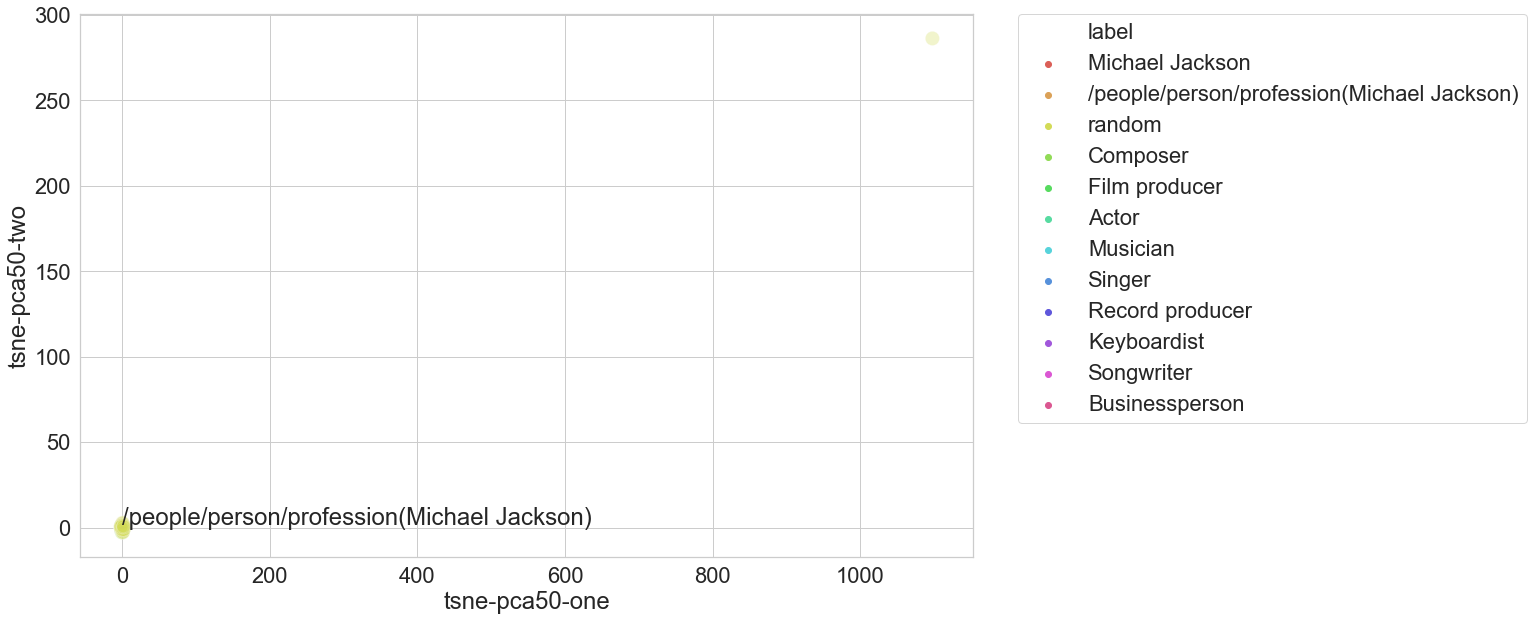
\includegraphics[width=0.7\textwidth, height=0.3\textheight]{t_sne_train_profession}
	\captionsetup{justification=centering}
	\caption{FB15k T-SNE: Triples about "Michael Jackson's" (subject) "profession" (predicate), pre HypER+ training. The legend lists all professions (objects) known to have have been performed by Michael Jackson. We can see most objects in the KG, regardless of type, clustered in the same embedding region. This includes the transformed subject-predicate vector,  "/people/person/profession(Michael Jackson)", used to take an inner product with an object. We expect this given Xavier \unskip~\citep{glorot2010understanding} intitialised entity and relation embeddings. }
\end{figure}

\begin{figure}[H]
   	\centering
    	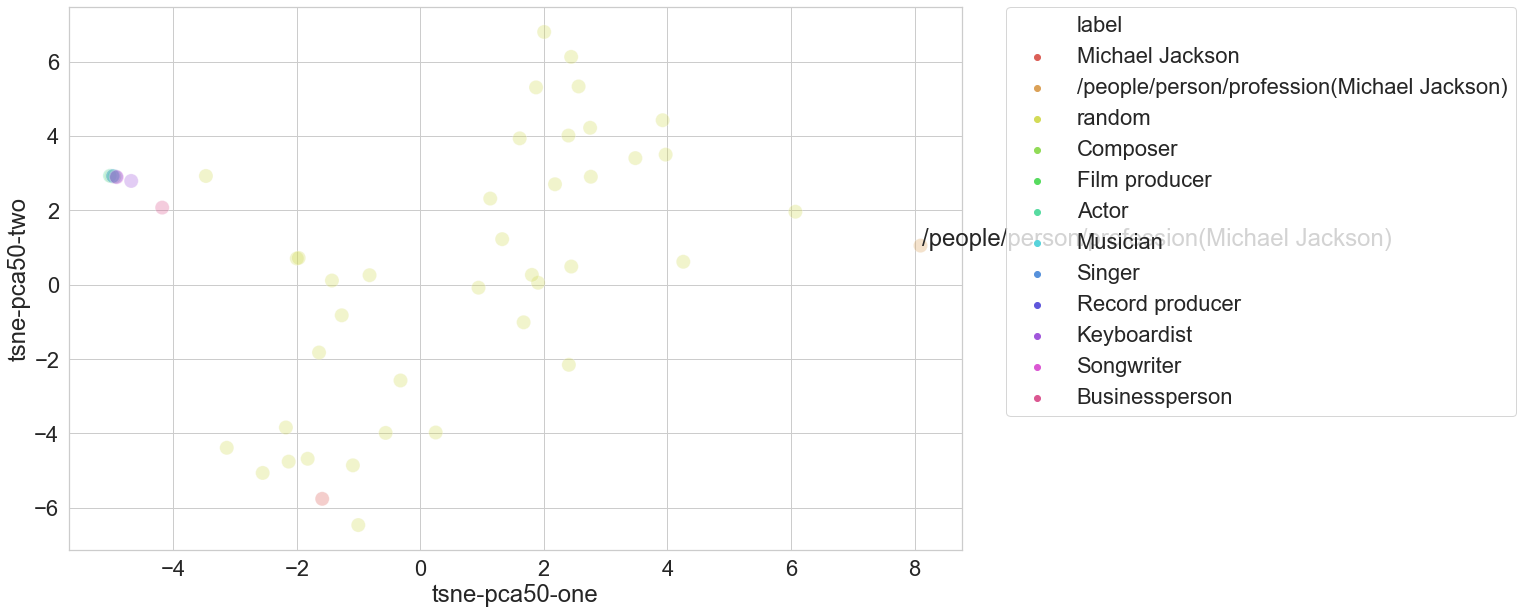
\includegraphics[width=0.7\textwidth, height=0.3\textheight]{t_sne_test_profession}
	\captionsetup{justification=centering}
	\caption{FB15k T-SNE: Triples about Michael Jackson's (subject) profession (predicate), post HypER+ training. Professions Michael Jackson is known to have performed are now all clustered within the same embedding region. This indicates the model has built some conceptual understanding around the objects.}
\end{figure}

\begin{figure}[H]
   	\centering
    	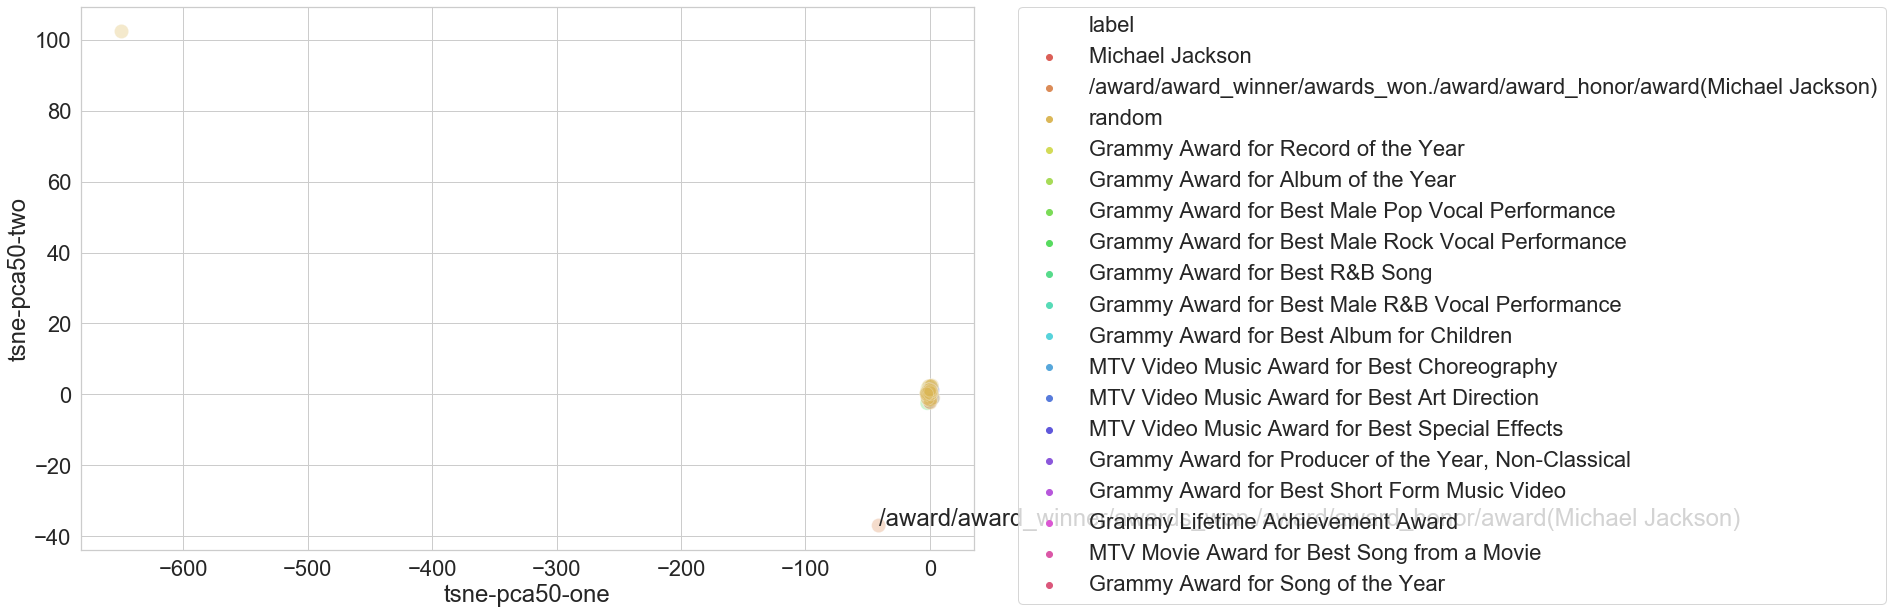
\includegraphics[width=0.7\textwidth, height=0.3\textheight]{t_sne_train_award}
	\captionsetup{justification=centering}
	\caption{FB15k T-SNE: Triples about "Michael Jackson's" (subject) "awards" (predicate), pre HypER+ training. The legend lists all awards (objects) known to have have been won by Michael Jackson. Once again we can see most objects in the KG, regardless of type, clustered in the same embedding region.}
\end{figure}

\begin{figure}[H]
   	\centering
    	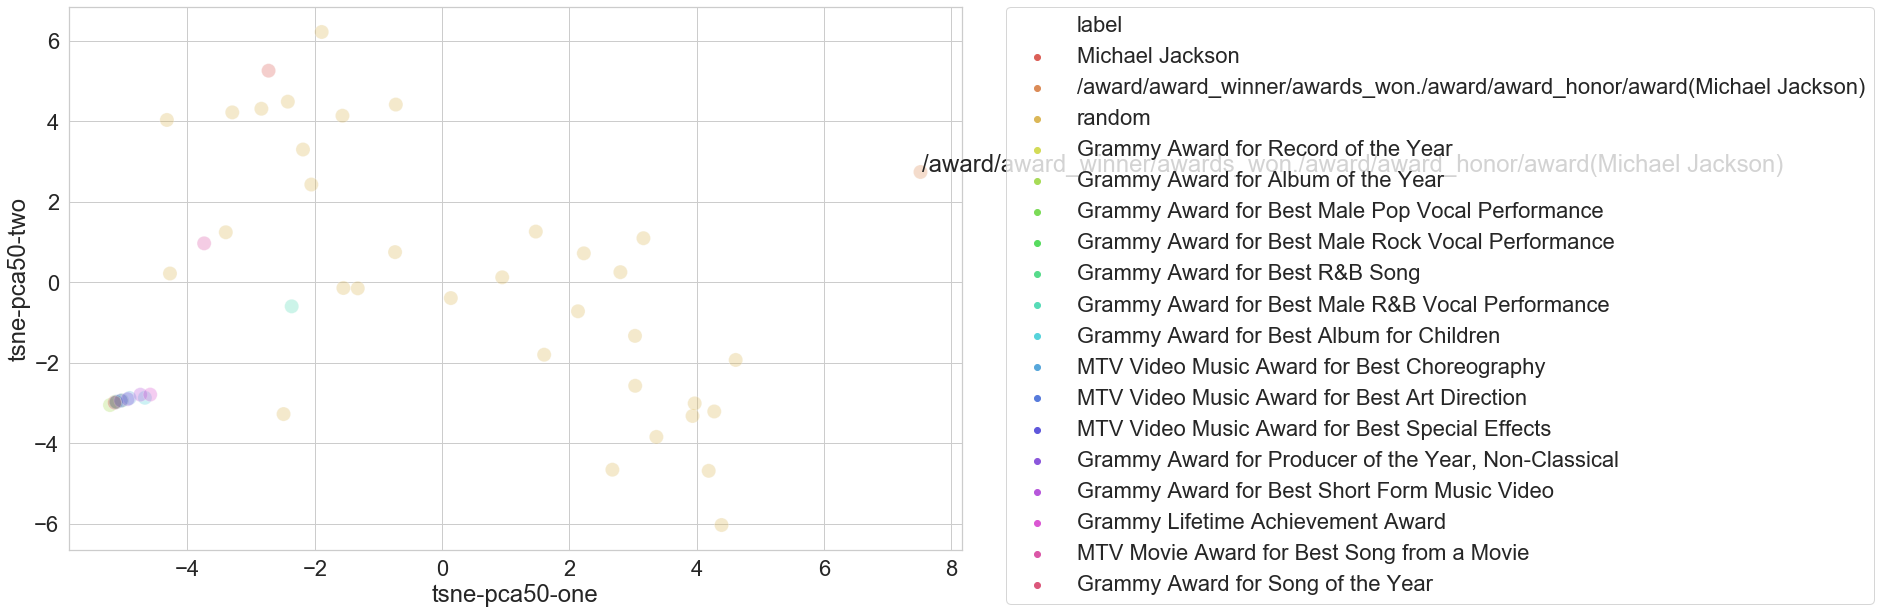
\includegraphics[width=0.7\textwidth, height=0.3\textheight]{t_sne_test_award}
	\captionsetup{justification=centering}
	\caption{FB15k T-SNE: Triples about "Michael Jackson's" (subject) "awards" (predicate), post HypER+ training. Awards Michael Jackson is known to have won are now somewhat clustered within the same embedding region. This indicates the model has built some conceptual understanding around the objects, and attempts to account for sub-domain differences, as well conceptual differences between the awards. For example, the "MTV Movie Award for Best Song from a Movie" is located in a region relatively far from all the "Music"-related awards. }
\end{figure}


%********************************** %HypER+ with Pre-Trained Word Embeddings  **************************************

\section{HypER+ with pre-trained word vectors}

\subsection{Baseline training algorithm}
\textbf{Model summary.} We extend HypER+ to make use of pre-trained word vectors from the GloVe \unskip ~\citep{pennington2014glove} language model. This model replaces Xavier initailised entity and relation embeddings with aggregated GloVe embeddings. The model is also trained using the binary cross-entropy loss. \par

\noindent \textbf{Experimental setup.} We use the following benchmark datasets.\ WN18RR is a subset of WN18, created by Dettmers et al. \unskip~\citep{dettmers2018convolutional} by removing the inverse relations from WN18. WN18RR contains $ 40, 943 $ entities and $ 11 $ relations. FB15k-237 was created by Toutanova et al. \unskip~\citep{toutanova2015observed}, noting that the validation and test sets of FB15k and WN18 contain the inverse of many relations present in the training set, making it easy for simple models to do well. FB15k-237 is a subset of FB15k with the inverse relations removed. It contains $ 14, 541 $ entities and $ 237 $ relations. Visualisations of the respective KGs, as well as a sample of RDF triple encoded facts, are presented in Figures 4.28 to 4.31. Property counts for the respective KGs are presented in Tables 4.10 and 4.11. \par. 

\begin{figure}[H]
   	\centering
    	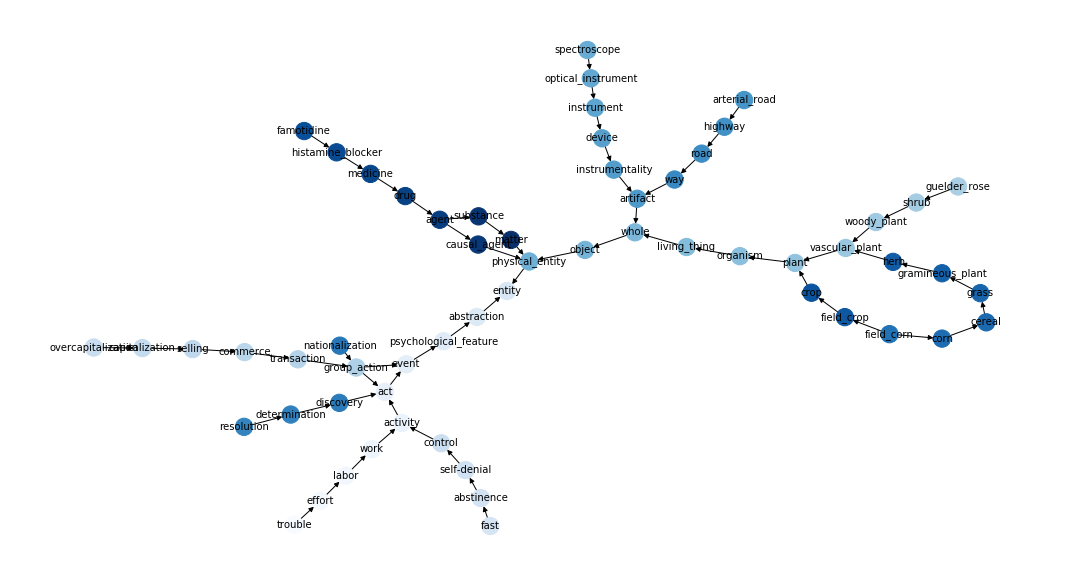
\includegraphics[width=0.9\textwidth, height=0.5\textwidth]{WN18RR_Graph}
	\captionsetup{justification=centering}
	\caption{A subset of WN18RR facts structured as a KG. Entities are nodes, and relations are edges, where a fact is encoded as an RDF triple.}
\end{figure}

\begin{figure}[H]
   	\centering
    	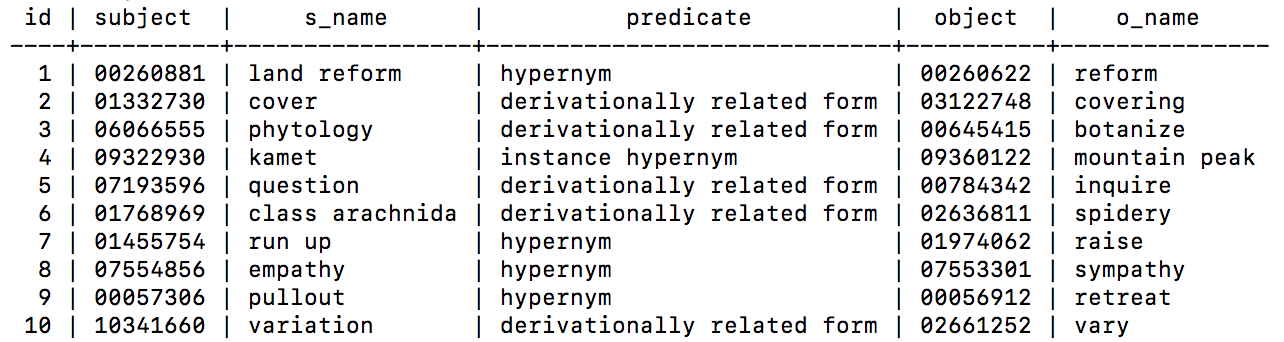
\includegraphics[width=0.9\textwidth, height=0.3\textwidth]{wn18rr_fact_sample}
	\captionsetup{justification=centering}
	\caption{A sample of RDF triples from the WN18RR KG.}
\end{figure}

\begin{figure}[H]
   	\centering
    	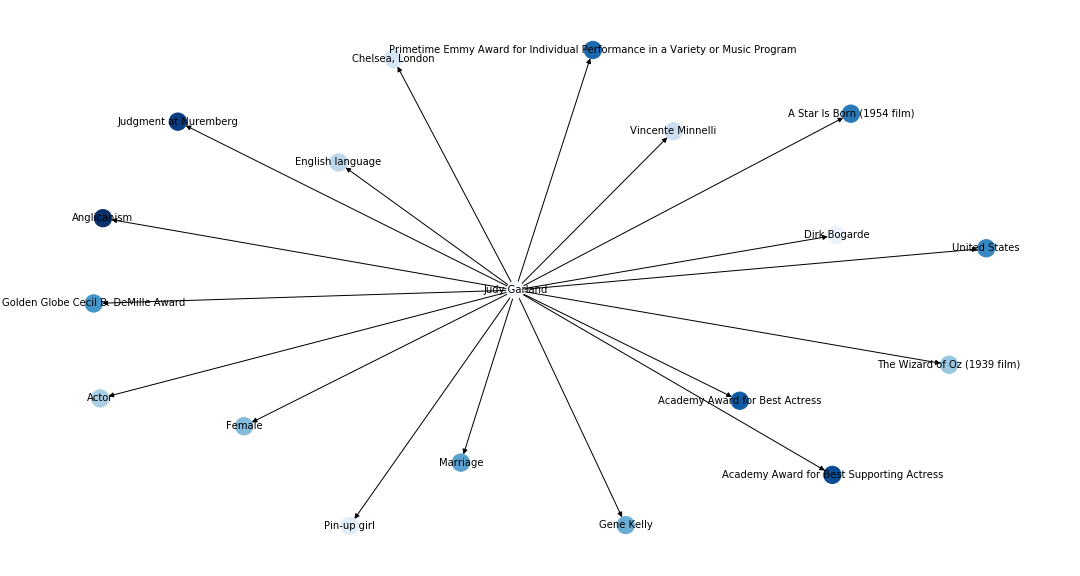
\includegraphics[width=0.9\textwidth, height=0.5\textwidth]{FB15k-237_Graph}
	\captionsetup{justification=centering}
	\caption{A subset of FB15k-237 facts structured as a KG. Entities are nodes, and relations are edges, where a fact is encoded as an RDF triple.}
\end{figure}

\begin{figure}[H]
   	\centering
    	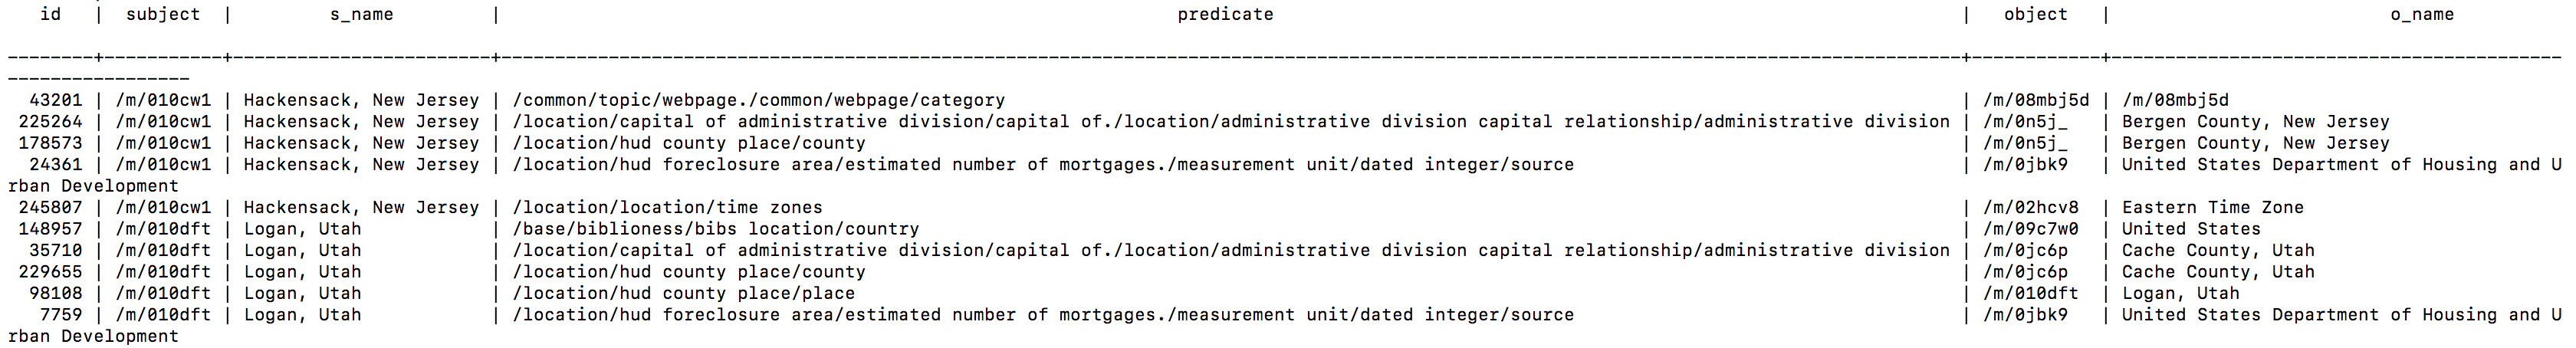
\includegraphics[width=1.0\textwidth, height=0.3\textwidth]{fb15k_237_fact_sample}
	\captionsetup{justification=centering}
	\caption{A sample of RDF triples from the FB15k-237 KG.}
\end{figure}

\noindent We used the PyTorch framework to implement the model.\ This model is built on top of the HypER+ model introduced in Section 4.2.2.\ Pre-trained GloVe word vectors are used to initialise entity and relational embeddings for model training.\ These embeddings are dynamically adjusted during the training process to generate latent representations specific to the KG. \par

\begin{table}[H]
	\parbox{.5\linewidth}{
		\centering
		\begin{tabular}{lllllllllll}
  			\textbf{Property} & \textbf{Count}  \\
  			\hline
  			Entities & 40,943  \\
  			Relations & 11  \\
  			Triples & 93,003 \\
			&
		\end{tabular}
		\captionsetup{justification=centering}
		\caption{Counts of WN18RR KG elements.}
		}
	\hfill
	\parbox{.5\linewidth}{
		\centering
		\begin{tabular}{lllllllllll}
  			\textbf{Property} & \textbf{Count}  \\
  			\hline
  			Entities & 14,541   \\
  			Relations & 237  \\
  			Triples & 310,116  \\
			&
		\end{tabular}
		\captionsetup{justification=centering}
		\caption{Counts of FB15k-237 KG elements.}
		}
\end{table}

%********************************** %Predicate **************************************

\noindent Summary statistics of the respective KG RDF formalism are presented in Figures 4.32 to 4.35, and Tables 4.22 and 4.27.

\begin{figure}[H]
   	\centering
    	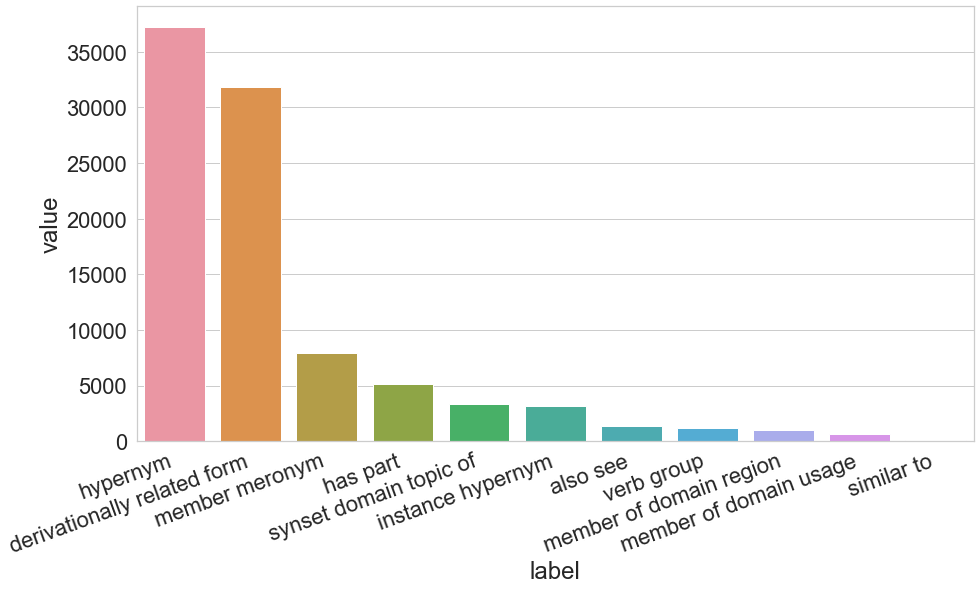
\includegraphics[width=0.7\textwidth, height=0.2\textheight]{WN18RR_Predicate_Counts}
	\captionsetup{justification=centering}
	\caption{WN18RR predicate distribution in KG facts.}
\end{figure}

\begin{table}[H]
		\centering
		\begin{tabular}{lllllllllll}
  			\textbf{Statistic} & \textbf{Value}  \\
  			\hline
			Count & 11 \\
			Max & 37,221  \\
			Min & 86 \\
  			Median & 3150  \\
  			IQR & 5433.5  \\
			&
		\end{tabular}
		\caption{WN18RR predicate statistics.}
\end{table}

\begin{figure}[H]
   	\centering
    	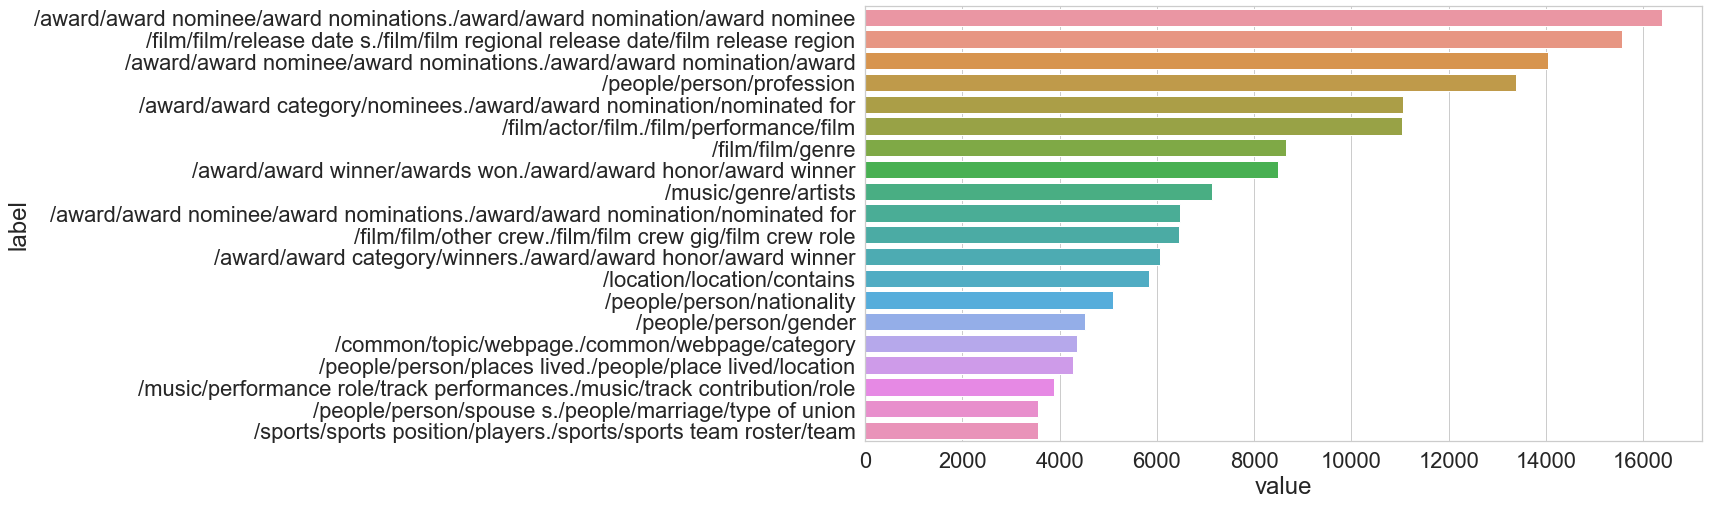
\includegraphics[width=1.0\textwidth, height=0.3\textheight]{FB15k-237_Predicate_Counts}
	\captionsetup{justification=centering}
	\caption{FB15k-237 predicate distribution in KG facts.}
\end{figure}

\begin{table}[H]
		\centering
		\begin{tabular}{lllllllllll}
  			\textbf{Statistic} & \textbf{Value}  \\
  			\hline
			Count & 237 \\
			Max & 16,391 \\
			Min & 45  \\
  			Median & 426  \\
  			IQR & 819 \\
			&
		\end{tabular}
		\caption{FB15k-237 predicate statistics.}
\end{table}

%********************************** %Subject **************************************

\begin{figure}[H]
	\begin{subfigure}[b]{.5\linewidth}
   		\centering
    		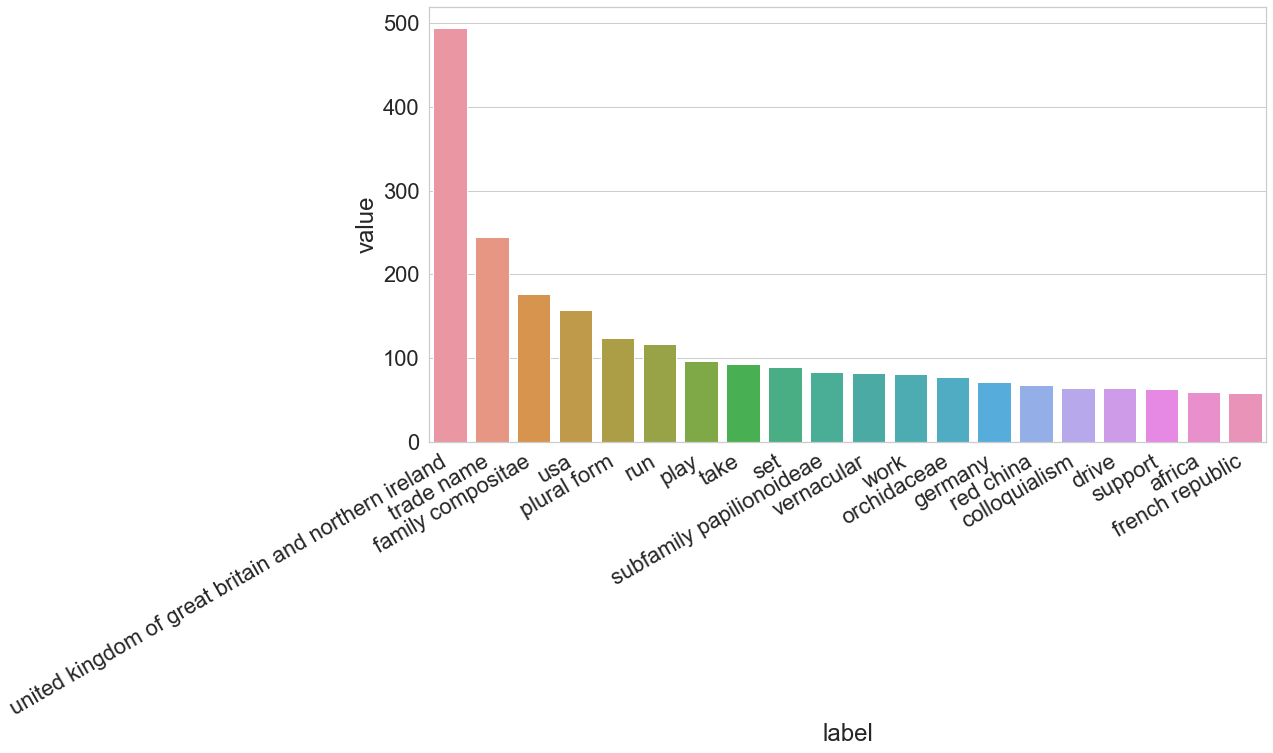
\includegraphics[width=1.0\linewidth, height=0.7\linewidth]{WN18RR_Subject_Counts}
		\captionsetup{justification=centering}
		\caption{WN18RR}
	\end{subfigure}
	\begin{subfigure}[b]{.5\linewidth}
   		\centering
		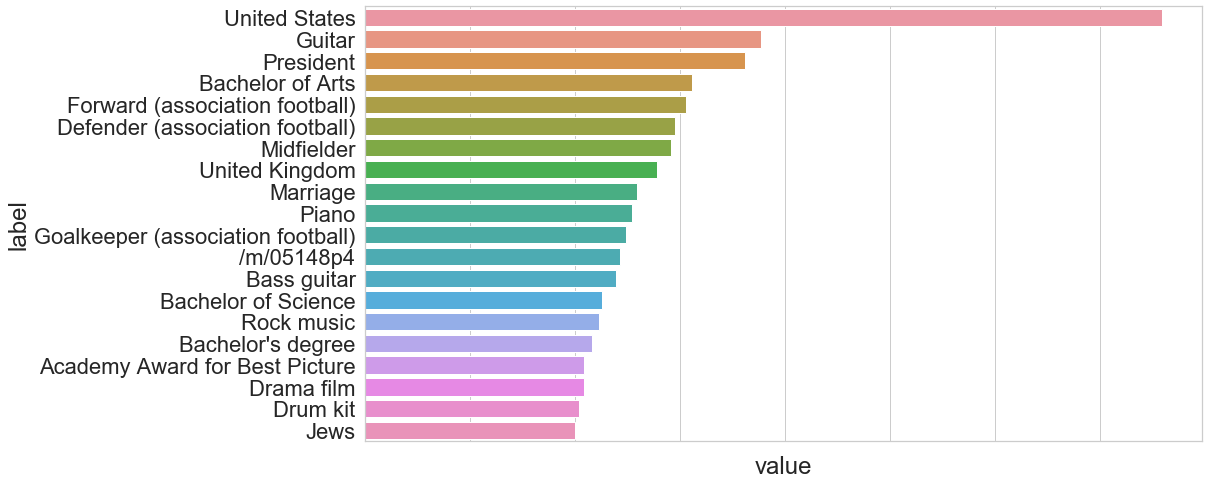
\includegraphics[width=1.0\linewidth, height=0.7\linewidth]{FB15k-237_Subject_Counts}
		\captionsetup{justification=centering}
		\caption{FB15k-237}
	\end{subfigure}
	\captionsetup{justification=centering}
	\caption{KG subject distribution. The number of times each subject takes part in a KG fact.}
\end{figure}

\begin{table}[H]
	\parbox{.5\linewidth}{
		\centering
		\begin{tabular}{lllllllllll}
  			\textbf{Statistic} & \textbf{Value}  \\
  			\hline
			Count & 32,349 \\
			Max & 494 \\
			Min & 1 \\
  			Median & 2 \\
  			IQR & 2 \\
			&
		\end{tabular}
		\caption{WN18RR subject statistics.}
		}
	\hfill
	\parbox{.5\linewidth}{
		\centering
		\begin{tabular}{lllllllllll}
  			\textbf{Statistic} & \textbf{Value}  \\
  			\hline
			Count &13,891 \\
			Max & 1,518 \\
			Min & 1 \\
  			Median & 16 \\
  			IQR & 20 \\
			&
		\end{tabular}
		\caption{FB15k-237 subject statistics.}
		}
\end{table}

%********************************** %Object **************************************

\begin{figure}[H]
	\begin{subfigure}[b]{.5\linewidth}
   		\centering
    		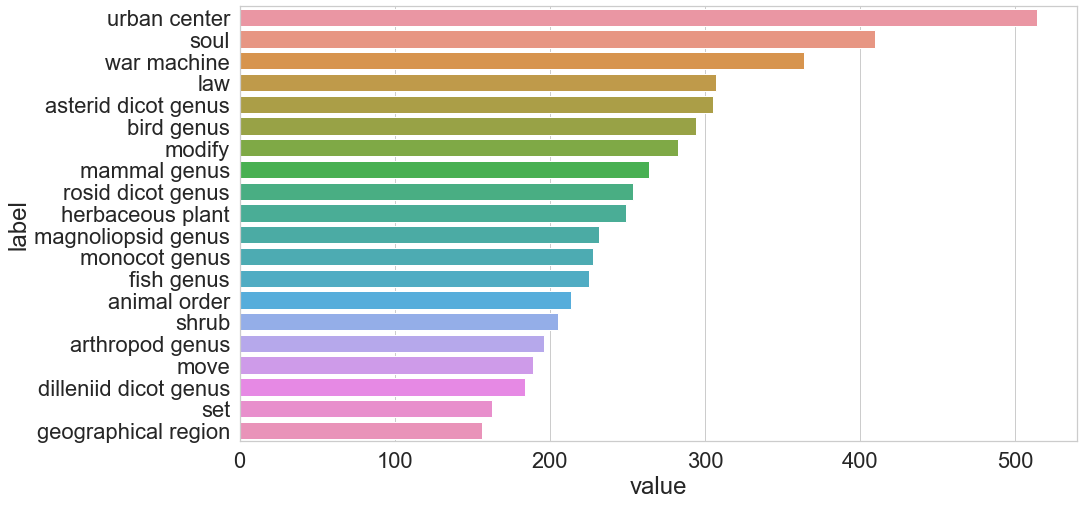
\includegraphics[width=1.0\linewidth, height=0.7\linewidth]{WN18RR_Object_Counts}
		\captionsetup{justification=centering}
		\caption{WN18RR}
	\end{subfigure}
	\begin{subfigure}[b]{.5\linewidth}
   		\centering
		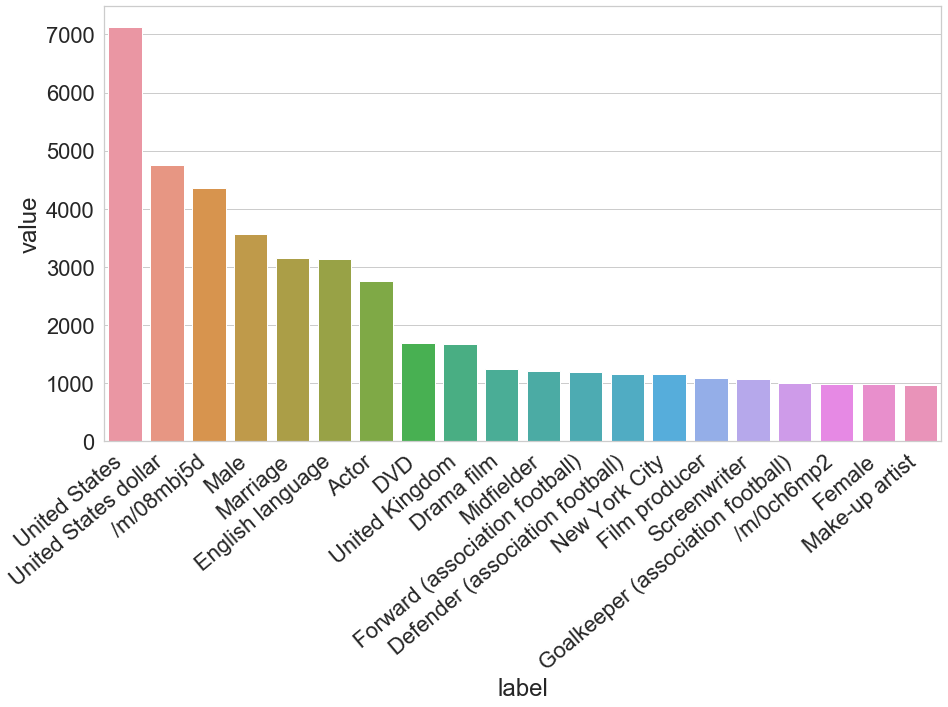
\includegraphics[width=1.0\linewidth, height=0.7\linewidth]{FB15k-237_Object_Counts}
		\captionsetup{justification=centering}
		\caption{FB15k-237}
	\end{subfigure}
	\captionsetup{justification=centering}
	\caption{KG object distribution. The number of times each subject takes part in a KG fact.}
\end{figure}

\begin{table}[H]
	\parbox{.5\linewidth}{
		\centering
		\begin{tabular}{lllllllllll}
  			\textbf{Statistic} & \textbf{Value}  \\
  			\hline
			Count & 26,162 \\
			Max & 514 \\
			Min & 1 \\
  			Median & 1 \\
  			IQR & 2 \\
			&
		\end{tabular}
		\caption{WN18RR object statistics.}
		}
	\hfill
	\parbox{.5\linewidth}{
		\centering
		\begin{tabular}{lllllllllll}
  			\textbf{Statistic} & \textbf{Value}  \\
  			\hline
			Count & 13,504 \\
			Max & 7,124 \\
			Min & 1 \\
  			Median & 10 \\
  			IQR & 16 \\
			&
		\end{tabular}
		\caption{FB15k-237 object statistics.}
		}
\end{table}

\noindent For WN18RR, it can be seen that predicates are skewed toward the relations "hypernym" and "derivationally related from", with a maximum of $ 37, 221 $ occurring, and an IQR of $ 5433.5 $ and $ 819 $ respectively. FB15k-237 predicates are skewed toward the film relation. \par

\noindent WN18RR and FB15k-237 subjects are somewhat uniform aside from a small number of high occurring entities, with the median number of occurrences being $ 2 $ and $ 16 $ respectively, and with an IQR of $ 2 $ and $ 20 $ respectively. WN18RR object occurrences are also somewhat uniform, while FB15k-237 object occurrences are skewed, with the "United States" partaking in the highest number of triples. This is in comparison to a median object occurrence of $ 1 $ and $ 10 $, and an IQR of $ 2 $ and $ 16 $ respectively. \par

\noindent The WN18RR dataset is split into a training, validation and test set of $ 86, 835 \; (93.368 \%) $, $ 3, 034 \; (3.262 \%) $ and $ 3, 134\; (3.37 \%) $ triples respectively.\ And the FB15k-237 dataset is split into a training, validation and test set of $ 272, 115 \; (87.746 \%) $, $ 17, 535 \; (5.654 \%) $ and $ 20, 466 \; (6.599 \%) $ triples respectively. \par


%********************************** %Pre-Trained Word Embeddings **************************************

\noindent The model was trained on Google Cloud Platform, on an N1 series instance with  8 CPU cores, 30GB RAM, 512GB SSD and an Nvidia Tesla P100 GPU. We train the respective models for $ 500 $ epoch, and evaluate them using the standard link prediction benchmarks discussed earlier. \par 

\noindent \textbf{Code to reproduce.} In the interest of reproducibility, all code needed to train and test the models in this section can be found at the following links. \newline
Baseline: \url{https://github.com/xhosaBoy/HypER-baseline} \newline
HypER+ with GloVe: \url{https://github.com/xhosaBoy/HypER-Pretrained-Word-Vectors} \par

\noindent \textbf{Link prediction results.} The cost and suite of current standard link prediction benchmark metrics, including Hit@10, Hit@3, Hit@1, Mean Rank and Mean Reciprocal Rank, are used to compare the HypER+ model without pre-trained embeddings, against the HypER baseline model, as well as against the HypER+ model without pre-trained embeddings, against the HypER+ model with pre-trained embeddings. The results are presented in Figures 4.18 and 4.23. as well as Tables 4.18 and 4.19. \par

%********************************** %Cost **************************************

\bigskip

\begin{figure}[H]
	\begin{subfigure}[b]{.5\linewidth}
   		\centering
    		\includegraphics[width=1.0\linewidth, height=0.6\linewidth]{WN18RR_Cost_Results}
		\captionsetup{justification=centering}
		\caption{WN18RR: HypER versus HypER+}
	\end{subfigure}
	\begin{subfigure}[b]{.5\linewidth}
   		\centering
		\includegraphics[width=1.0\linewidth, height=0.6\linewidth]{FB15k-237_Cost_Results}
		\captionsetup{justification=centering}
		\caption{FB15k-237: HypER versus HypER+}
	\end{subfigure}
	\captionsetup{justification=centering}
	\caption{Cost versus epoch for the respective KG. There is a large difference between the HypER (baseline) and HypER+ (hypothesis) costs, where the hypothesis cost is approximately half the baseline cost on both KGs. The FB15k-237 costs exhibit similar behaviour as that discussed earlier, dropping sharply in the first 10 epochs, before rising and plateauing. Once again this could be attributed to small probabilities first computed by the models, before becoming more confident with larger probabilities. And once again the FB15k-237 cost is also higher than the WN18RR cost, this may also be due their respective KG size and complexity.}
\end{figure}

\begin{figure}[H]
	\begin{subfigure}[b]{.5\linewidth}
   		\centering
    		\includegraphics[width=1.0\linewidth, height=0.6\linewidth]{WN18RR_Cost_Results_ptwv}
		\captionsetup{justification=centering}
		\caption{WN18RR: HypER+ versus \\ HypER+ with Pre-Trained Embeddings}
	\end{subfigure}
	\begin{subfigure}[b]{.5\linewidth}
   		\centering
		\includegraphics[width=1.0\linewidth, height=0.6\linewidth]{FB15k-237_Cost_Results_ptwv}
		\captionsetup{justification=centering}
		\caption{FB15k-237: HypER+ versus \\ HypER+ with Pre-Trained Embeddings}
	\end{subfigure}
	\captionsetup{justification=centering}
	\caption{Cost versus epoch for the respective KG. Interestingly the baseline cost (HypER+) is consistently lower than the hypothesis cost (HypER+ with pre-trained word embeddings), on both KGs. This may be attributed to the domain knowledge accumulated during language model building. This knowledge may be optimised for the corpus on which the language model was trained, and not align well with the respective KG domains.}
\end{figure}


%********************************** %Hits@10 **************************************

\begin{figure}[H]
	\begin{subfigure}[b]{.5\linewidth}
   		\centering
    		\includegraphics[width=1.0\linewidth, height=0.6\linewidth]{WN18RR_hits_at_10_Results}
		\captionsetup{justification=centering}
		\caption{WN18RR: HypER versus HypER+}
	\end{subfigure}
	\begin{subfigure}[b]{.5\linewidth}
   		\centering
		\includegraphics[width=1.0\linewidth, height=0.6\linewidth]{FB15k-237_hits_at_10_Results}
		\captionsetup{justification=centering}
		\caption{FB15k-237: HypER versus HypER+}
	\end{subfigure}
	\captionsetup{justification=centering}
	\caption{Hits@10 versus epoch for the respective KG. There is once again hardly any difference between the hypothesis and baseline models for the WN18RR KG. The hypothesis model marginally outperforms the baseline on the FB15k-237 KG. There is also a pronounced difference between training set performance and validation set performance on both KGs. The bears the impact inverse relations have on WN18 and FB15k respectively, as discussed earlier.}
\end{figure}

\begin{figure}[H]
	\begin{subfigure}[b]{.5\linewidth}
   		\centering
    		\includegraphics[width=1.0\linewidth, height=0.6\linewidth]{WN18RR_hits_at_10_Results_ptwv}
		\captionsetup{justification=centering}
		\caption{WN18RR: HypER+ versus \\ HypER+ with Pre-Trained Embeddings}
	\end{subfigure}
	\begin{subfigure}[b]{.5\linewidth}
   		\centering
		\includegraphics[width=1.0\linewidth, height=0.6\linewidth]{FB15k-237_hits_at_10_Results_ptwv}
		\captionsetup{justification=centering}
		\caption{FB15k-237: HypER+ versus \\ HypER+ with Pre-Trained Embeddings}
	\end{subfigure}
	\captionsetup{justification=centering}
	\caption{Hits@10 versus epoch for the respective KG. The hypothesis significantly outperforms the baseline on the WN18RR KG. The hypothesis only marginally outperforms the baseline on the FB15k-237 KGb. This suggests pre-trained embeddings have more of an impact on smaller KGs, where relations are likely to be more sparse, making it harder to build entity and relation conceptual understanding.}
\end{figure}


%********************************** %Hits@3 **************************************

\begin{figure}[H]
	\begin{subfigure}[b]{.5\linewidth}
   		\centering
    		\includegraphics[width=1.0\linewidth, height=0.6\linewidth]{WN18RR_hits_at_3_Results}
		\captionsetup{justification=centering}
		\caption{WN18RR: HypER versus HypER+}
	\end{subfigure}
	\begin{subfigure}[b]{.5\linewidth}
   		\centering
		\includegraphics[width=1.0\linewidth, height=0.6\linewidth]{FB15k-237_hits_at_3_Results}
		\captionsetup{justification=centering}
		\caption{FB15k-237: HypER versus HypER+}
	\end{subfigure}
	\captionsetup{justification=centering}
	\caption{Hits@3 versus epoch for the respective KG. The hypothesis only marginally outperforms the baseline on both KGs once accuracy constraints become more robust.}
\end{figure}

\begin{figure}[H]
	\begin{subfigure}[b]{.5\linewidth}
   		\centering
    		\includegraphics[width=1.0\linewidth, height=0.6\linewidth]{WN18RR_hits_at_3_Results_ptwv}
		\captionsetup{justification=centering}
		\caption{WN18RR: HypER+ versus \\ HypER+ with Pre-Trained Embeddings}
	\end{subfigure}
	\begin{subfigure}[b]{.5\linewidth}
   		\centering
		\includegraphics[width=1.0\linewidth, height=0.6\linewidth]{FB15k-237_hits_at_3_Results_ptwv}
		\captionsetup{justification=centering}
		\caption{FB15k-237: HypER+ versus \\ HypER+ with Pre-Trained Embeddings}
	\end{subfigure}
	\captionsetup{justification=centering}
	\caption{Hits@3 versus epoch for the respective KG. Even with pre-trained embedding initialisation, the hypothesis once again only marginally outperforms the baseline on both KG validation sets. There is a pronounced difference between performance on the FB15k-237 training set. This difference may once again be due to pre-trained embedding domain alignment with the language model. Efficient regularisation ensures superior hypothesis performance on the validation set.}
\end{figure}


%********************************** %Hits@1 **************************************

\begin{figure}[H]
	\begin{subfigure}[b]{.5\linewidth}
   		\centering
    		\includegraphics[width=1.0\linewidth, height=0.6\linewidth]{WN18RR_hits_at_1_Results}
		\captionsetup{justification=centering}
		\caption{WN18RR: HypER versus HypER+}
	\end{subfigure}
	\begin{subfigure}[b]{.5\linewidth}
   		\centering
		\includegraphics[width=1.0\linewidth, height=0.6\linewidth]{FB15k-237_hits_at_1_Results}
		\captionsetup{justification=centering}
		\caption{FB15k-237: HypER versus HypER+}
	\end{subfigure}
	\captionsetup{justification=centering}
	\caption{Hits@1 versus epoch for the respective KG. The is no discernible difference in performance between the hypothesis and baseline on the WN18RR KG. The hypothesis marginally outperforms the baseline on the FB15k-237 KG. This suggests the impact of covariate shift is less significant on smaller, less complex datasets.}
\end{figure}

\begin{figure}[H]
	\begin{subfigure}[b]{.5\linewidth}
   		\centering
    		\includegraphics[width=1.0\linewidth, height=0.6\linewidth]{WN18RR_hits_at_1_Results_ptwv}
		\captionsetup{justification=centering}
		\caption{WN18RR: HypER+ versus \\ HypER+ with Pre-Trained Embeddings}
	\end{subfigure}
	\begin{subfigure}[b]{.5\linewidth}
   		\centering
		\includegraphics[width=1.0\linewidth, height=0.6\linewidth]{FB15k-237_hits_at_1_Results_ptwv}
		\captionsetup{justification=centering}
		\caption{FB15k-237: HypER+ versus \\ HypER+ with Pre-Trained Embeddings}
	\end{subfigure}
	\captionsetup{justification=centering}
	\caption{Hits@1 versus epoch for the respective KG. Once more there is no discernible difference in performance between the hypothesis and baseline, this time on both KGs. This suggests semantic information advantages gained from pre-trained embeddings are not aligned enough with the respective KGs at this level of accuracy robustness.}
\end{figure}

%********************************** %Mean rank **************************************

\begin{figure}[H]
	\begin{subfigure}[b]{.5\linewidth}
   		\centering
    		\includegraphics[width=1.0\linewidth, height=0.6\linewidth]{WN18RR_mean_rank_Results}
		\captionsetup{justification=centering}
		\caption{WN18RR: HypER versus HypER+}
	\end{subfigure}
	\begin{subfigure}[b]{.5\linewidth}
   		\centering
		\includegraphics[width=1.0\linewidth, height=0.6\linewidth]{FB15k-237_mean_rank_Results}
		\captionsetup{justification=centering}
		\caption{FB15k-237: HypER versus HypER+}
	\end{subfigure}
	\captionsetup{justification=centering}
	\caption{Mean Rank versus epoch for the respective KG. The hypothesis is outperformed by the baseline on the WN18RR KG, however the hypothesis outperforms the baseline on the FB15k-237 KG. The impact of KG size and complexity on covariate shift seems to drive this behaviour, where relational batch normalisation is very effective at inducing good latent representations for relations, resulting in a consistently higher rank for the correct prediction.}
\end{figure}

\begin{figure}[H]
	\begin{subfigure}[b]{.5\linewidth}
   		\centering
    		\includegraphics[width=1.0\linewidth, height=0.6\linewidth]{WN18RR_mean_rank_Results_ptwv}
		\captionsetup{justification=centering}
		\caption{WN18RR: HypER+ versus \\ HypER+ with Pre-Trained Embeddings}
	\end{subfigure}
	\begin{subfigure}[b]{.5\linewidth}
   		\centering
		\includegraphics[width=1.0\linewidth, height=0.6\linewidth]{FB15k-237_mean_rank_Results_ptwv}
		\captionsetup{justification=centering}
		\caption{FB15k-237: HypER+ versus \\ HypER+ with Pre-Trained Embeddings}
	\end{subfigure}
	\captionsetup{justification=centering}
	\caption{Mean Rank versus epoch for the respective KG. There is a stark difference in performance between the hypothesis and baseline on the WN18RR KG. Pre-trained embeddings are very effective at providing semantic information that can be used to produce good predictions for smaller, less complex KGs. The difference is less pronounced on the FB15k-237 KG, however is still significant.}
\end{figure}



%********************************** %Mean reciprocal rank **************************************

\begin{figure}[H]
	\begin{subfigure}[b]{.5\linewidth}
   		\centering
    		\includegraphics[width=1.0\linewidth, height=0.6\linewidth]{WN18RR_mean_reciprocal_rank_Results}
		\captionsetup{justification=centering}
		\caption{WN18RR: HypER versus HypER+}
	\end{subfigure}
	\begin{subfigure}[b]{.5\linewidth}
   		\centering
		\includegraphics[width=1.0\linewidth, height=0.6\linewidth]{FB15k-237_mean_reciprocal_rank_Results}
		\captionsetup{justification=centering}
		\caption{FB15k-237: HypER versus HypER+}
	\end{subfigure}
	\captionsetup{justification=centering}
	\caption{Mean Reciprocal Rank versus epoch for the respective KG.There is no discernible difference in performance on the WN18 KG, however the hypothesis marginally outperforms baseline is on the FB15k-237 KG.}
\end{figure}

\begin{figure}[H]
	\begin{subfigure}[b]{.5\linewidth}
   		\centering
    		\includegraphics[width=1.0\linewidth, height=0.6\linewidth]{WN18RR_mean_reciprocal_rank_Results_ptwv}
		\captionsetup{justification=centering}
		\caption{WN18RR: HypER+ versus \\ HypER+ with Pre-Trained Embeddings}
	\end{subfigure}
	\begin{subfigure}[b]{.5\linewidth}
   		\centering
		\includegraphics[width=1.0\linewidth, height=0.6\linewidth]{FB15k-237_mean_reciprocal_rank_Results_ptwv}
		\captionsetup{justification=centering}
		\caption{FB15k-237: HypER+ versus \\ HypER+ with Pre-Trained Embeddings}
	\end{subfigure}
	\captionsetup{justification=centering}
	\caption{Mean Reciprocal Rank versus epoch for the respective KG. The hypothesis marginally outperforms the baseline on the WN18RR KG, and there is no discernible difference in performance on the FB15k-237 KG. This again suggests pre-trained embeddings having more of an impact on the WN18RR KG.}
\end{figure}


%********************************** %Test results **************************************

\begin{table}[H]
		\centering
		\begin{tabular}{lllllllllll}
  			\textbf{Model} & \textbf{H@10} & \textbf{H@3} & \textbf{H@1} & \textbf{MR} & \textbf{MRR} \\
  			\hline
  			DistMult \unskip~\citep{yang2014embedding} & .490 & .440 & .390 & 5110 & .430 \\
  			ComplEx \unskip~\citep{trouillon2016complex} & .510 & .460 & .410 & 5261 & .440 \\
  			Neural LP \unskip~\citep{yang2017differentiable} & - & - & - & - & - \\
			ConvE \unskip~\citep{dettmers2018convolutional} & .520 & .440 & .400 & 4187 & .430 \\
			HypER \unskip~\citep{balazevic2019hypernetwork} & .522 & .477 & .436 & 5798 & .465 \\
			HypER+ (ours) & .519 & .479 & \textbf{.438} & 7061 & .466 \\
  			\hline
  			HypER+ with pre-trained embeddings (ours) & \textbf{.578} & \textbf{.493} & .435 & \textbf{1063} & \textbf{.480} \\
			&
		\end{tabular}
		\captionsetup{justification=centering}
		\caption{Relation prediction test results on WN18RR. HypER+ with pre-trained word embeddings significantly outperforms both the HypER as well as HypER+ models. HypER+ outperforms HypER+ with pre-trained embeddings on the Hit@1 metric, consistent with the expectation of diminished impact of pre-trained embeddings at high levels of accuracy constraints. It should be note that there is a difference of $ 0.3 \% $ between all three models (HypER, HypER+ and HypER+ with pre-trained word embeddings), suggesting almost identical performance. The largest differences in performance occur at Hit@10 and Mean Rank, bearing the effectiveness of pre-trained embeddings at compensating for sparsity, however also highlighting how their significance diminishes at higher levels of accuracy. }
\end{table}

\begin{table}[H]
		\centering
		\begin{tabular}{lllllllllll}
  			\textbf{Model} & \textbf{H@10} & \textbf{H@3} & \textbf{H@1} & \textbf{MR} & \textbf{MRR} \\
  			\hline
  			DistMult \unskip~\citep{yang2014embedding} & .419 & .263 & .155 & 254 & .241 \\
  			ComplEx \unskip~\citep{trouillon2016complex} & .428 & .275 & .158 & 339 & .247 \\
  			Neural LP  \unskip~\citep{yang2017differentiable} & .408 & - & - & - & .250 \\
			ConvE \unskip~\citep{dettmers2018convolutional} & .501 & .356 & .237 & 244 & .325 \\
			HypER \unskip~\citep{balazevic2019hypernetwork} & .520 & .376 & .252 & 250 & .341 \\
			HypER+ (ours) & .516 & .368 & .245 & 268 & .335 \\
  			\hline
  			HypER+ with pre-trained embeddings (ours) & \textbf{.525} & \textbf{.379} & \textbf{.255} & \textbf{196} & \textbf{.345} \\
			&
		\end{tabular}
		\captionsetup{justification=centering}
		\caption{Relation prediction test results on FB15k-237. The HypER+ model with pre-trained embeddings achieves state-of-the-art (SOTA) performance across all metrics. Covariate shift seems to not be playing as meaningful a role, and pre-trained embeddings are providing a more meaningful contribution. This suggested by the HypER+ model's inferior performance to the HypER model. Strangely, this is inconsistent with training and validation set results, where HypER+ consistently outperforms HypER on FB15k-237. Using the quoted HypER test results, as opposed to reimplemented and verified test results may explain this inconsistency. There may be an implementation detail not used by the thesis author to achieve the quoted level of performance. This inconsistency aside, pre-trained embeddings remain effective at improving relation prediction performance on the FB15k-237 KG.}
\end{table}


%********************************** %Test Result Decomposition **************************************

\begin{figure}[H]
   	\centering
    	\includegraphics[width=0.7\textwidth, height=0.3\textheight]{WN18RR_relational_performance_results}
	\captionsetup{justification=centering}
	\caption{WN18RR Hit@ 1 Predicate Performance. The relation predication performance of the HypER+ model with pre-trained embeddings. The model performs well with synonym relation types, however performs poorly with compositional and hierarchical relations. This may be due to the inherent similarity and analogy in concepts, where as compositions and hierarchies can be defined by strict rules. Perhaps, more simply, this is due to the number of test set samples for each relation, where higher numbers increase the prediction error rate.}
\end{figure}

\begin{table}[H]
	\centering
	\resizebox{1.0\columnwidth}{!}{
	\begin{tabular}{lllllllllll}
  		\textbf{Subject} & \textbf{Predicate} & \textbf{Object Target} & \textbf{Object Prediction} \\
  		\hline
  		usa & has part & colorado & missouri river \\
  		spain & has part & cadiz & jerez de la frontera \\
  		kilobyte & has part & computer memory unit & word \\
		electromagnetic spectrum & has part & actinic ray & radio spectrum \\
		systema respiratorium & has part & respiratory tract & respiratory organ \\
		respiratory organ & has part & nsa & defense advanced research projects agency \\
		africa & has part & nigeria & senegal \\
  		antigen & has part & substance & epitope \\
		amphitheatre & has part & theatre & tiered seat \\
		indian ocean & has part & mauritius & antarctic ocean \\
		&
	\end{tabular}
	}
	\captionsetup{justification=centering}
	\caption{Qualitative Hit@1 Test results on WN18RR. The table presents a set of questions posed to the HypER+ with pre-trained embeddings model. The "Object Target" is the expected answer, and the "Object Prediction" is the answer given by the model. The model demonstrates basic coneptual understanding, never making mistakes that would be considered "obvious" by humans. We would expect reasonable knowledge discovery utility from the model, when used jointly with information retrieval for open-domain question answering \unskip~\citep{chen2017reading}. }
\end{table}


%********************************** %Chapter Summary  **************************************

\section{Summary}

\textbf{NTN with optimised training algorithm.} We attempt to improve the NTN model by applying training algorithm optimisations including early stopping, the Adam optimiser and hyperparameter random search. The results indicate that there are potential performance gains to be realised simply through using training algorithm techniques known to improve performance. In this instance we see an accuracy gain of 6.2\%, across the WordNet and Freebase datasets. \par

\noindent \textbf{HypER+.} We compensate for possible covariate shift introduced by hypernetworks.\ The latent representation distribution drift of relations is pronounced enough that we are able to improve the Hit@1 accuracy of the original HypER model on average by 2.7\%, across the WN18 and FB15k KGs.\ We note graph modelling may be a worthwhile paradigm to explore for link prediction, given R-GCN's SOTA performance for Hit@10 accuracy on the WN18 KG. We also note the greater influence of relational normalisation on prediction performance for larger and more complex KGs. \par

\noindent \textbf{HypER+ with pre-trained word vectors.} Finally we extend HypER+ to make use of pre-trained GloVe word vectors.\ The semantic information inherent in these embeddings significantly improves relation prediction performance on sparse relational data. Their influence is somewhat reduced at higher levels of accuracy, where KG domain alignment becomes more important. Pre-trained word vectors also offer less utility for large and complex KGs, however still contribute an improvement to prediction. The combination of relation normalisation, and entity and relation embedding initialisation using pre-trained word vectors, addresses both the problems of data sparsity, as well as producing higher quality relational latent representations for large and complex datasets. As a result, HypER+ with pre-trained word vectors achieves SOTA performance on almost all standard link prediction benchmark metrics, across both the WN18RR and FB15k-237 KGs. 
